%This is a very basic  BE PROJECT PRELIMINARY template.

%############################################# 
%#########Author :  PROJECT###########
%#########COMPUTER ENGINEERING############


\documentclass[oneside,a4paper,12pt]{report}
%\usepackage{showframe}
%\hoffset = 8.9436619718309859154929577464789pt
%\voffset = 13.028169014084507042253521126761pt

\fancypagestyle{plain}{%
  \fancyhf{}
  \fancyfoot[CE]{AVCOE, Sangamner, Department of Computer Engineering 2023-24}
  \fancyfoot[RE]{\thepage}
}
\pagestyle{fancy}
\fancyhead{}
\renewcommand{\headrulewidth}{0pt}
\footskip = 0.625in
\cfoot{}
\rfoot{}

\usepackage[]{hyperref}
\usepackage{tikz}
\usetikzlibrary{arrows,shapes,snakes,automata,backgrounds,petri}

\usepackage{tabularx}

\usepackage[nottoc,notlot,notlof,numbib]{tocbibind}
\usepackage[titletoc]{appendix}
\usepackage{titletoc}
\renewcommand{\appendixname}{Annexure}
\renewcommand{\bibname}{References}

\setcounter{secnumdepth}{5}

\usepackage{float}
\usepackage{subcaption}
\usepackage{multirow}
\usepackage{amsmath}

\usepackage[ruled,vlined]{algorithm2e}

\begin{document}

\setlength{\parindent}{0mm}
\begin{center}
{\bfseries SAVITRIBAI PHULE PUNE UNIVERSITY \\}
 \vspace*{1\baselineskip}
{\bfseries A PRELIMINARY PROJECT REPORT ON \\}
 \vspace*{1\baselineskip}
{\bfseries \fontsize{16}{12} \selectfont Image Captioning System using Deep Neural Network based on Encoder-Decoder Framework. \\\vspace*{1\baselineskip}}
{\fontsize{12}{12} \selectfont SUBMITTED TO THE SAVITRIBAI PHULE PUNE UNIVERSITY, PUNE
IN THE PARTIAL FULFILLMENT OF THE REQUIREMENTS 
FOR THE AWARD OF THE DEGREE \\
\vspace*{2\baselineskip}}
{\bfseries \fontsize{14}{12} \selectfont 
\hspace{18 mm}BACHELOR OF ENGINEERING
\newline(Computer Engineering)(SEM-I) \\
\vspace*{1\baselineskip}} 
{\bfseries \fontsize{14}{12} \selectfont SUBMITTED BY \\ 
} 
\begin{center}
\bf{Group ID : A19}
\end{center}
\begin{flushleft}
\hspace{15mm}Mr. Mayur Sopan  Gadakh   \hspace{31 mm} Exam No: B190104240  \\
\hspace{15mm}Mr. Gaurav Bhima Chaudhari  \hspace{25 mm} Exam No: B190104219   \\
\hspace{15mm}Ms. Akanksha Bhausaheb Gaikwad   \hspace{15 mm} Exam No: B190104245 \\
\hspace{15mm}Ms. Shivanjali Anil Dhage \hspace{30 mm} Exam No: B190104229\\
\end{flushleft}
\vspace*{1\baselineskip}
{\bfseries \fontsize{14}{12} \selectfont Under The Guidance of \\  
\vspace*{2mm}} 
\bf{Dr. R. S. Gaikwad}\\

\includegraphics[width=100pt]{AVCOE_LOGO.png} \\
{\bfseries \fontsize{14}{12} \selectfont DEPARTMENT OF COMPUTER ENGINEERING \\
Amrutvahini College of Engineering, Sangamner\\
Amrutnagar, Ghulewadi - 422608 \\
2023-24
}
\end{center}

\newpage



\begin{figure}[ht]
\centering

\includegraphics[width=100pt]{AVCOE_LOGO.png}
\end{figure}


{\bfseries \fontsize{14}{12} \selectfont \centerline{AMRUTVAHINI COLLEGE OF ENGINEERING,SANGAMNER}
\centerline{DEPARTMENT OF COMPUTER ENGINEERING}
\vspace*{1\baselineskip}} 


{\bfseries \fontsize{16}{12} \selectfont \centerline{CERTIFICATE} 
\vspace*{1mm}}

\centerline{This is to certify that the Project Entitled}
\vspace{5mm}


{\bfseries \fontsize{14}{12} \selectfont \centerline{Image Captioning system using deep neural network based}
\vspace{0mm}}

{\bfseries \fontsize{14}{12} \selectfont \centerline{ on encoder-decoder framework.}

\vspace*{1mm}}

\centerline{Submitted by}
\vspace*{1mm}
\centerline{\bf{Group ID: A19}}  
\begin{flushleft}
\hspace{15mm}Mr. Mayur Sopan Gadakh   \hspace{31 mm} Exam No: B190104240  \\
\hspace{15mm}Mr. Gaurav Bhima Chaudhari  \hspace{25 mm} Exam No: B190104219   \\
\hspace{15mm}Ms. Akanksha Bhausaheb Gaikwad  \hspace{15 mm} Exam No:  B190104245  \\
\hspace{15mm}Ms. Shivanjali Anil Dhage \hspace{30 mm} Exam No: B190104229\\
\end{flushleft}
\vspace*{1mm} 
are bonafide students of this institute and the work has been carried out by them under the supervision of  Dr. R. S. Gaikwad and it is approved for the partial fulfillment of the requirement of Savitribai Phule Pune University, for the award of the degree of Bachelor of Engineering (Computer Engineering). \\\\
\bgroup
\def\arraystretch{0.7}
\begin{tabular}{c c }
\\
\\
Dr. R. S. Gaikwad &  \hspace{40 mm} Dr. R. G. Tambe / Dr. D. R. Patil \\								
Internal Guide   &  \hspace{40 mm} Project Coordinator \\
Dept. of Computer Engg.  &	\hspace{40 mm}Dept. of Computer Engg.  \\
\end{tabular}
 \vspace*{1.5\baselineskip}                     
                                                   
\begin{tabular}{c c }
\\
Dr. S. K. Sonkar &  \hspace{50 mm} Dr. M.A. Venkatesh \\								
H.O.D.   &  \hspace{50 mm} Principal \\
Dept. of Computer Engg.  &	\hspace{50 mm}AVCOE Sangamner  \\
\end{tabular}
%}

\newpage

\begin{center}
{\bfseries SAVITRIBAI PHULE PUNE UNIVERSITY \\}
\end{center}

\begin{figure}[ht]
\centering

\includegraphics[width=150pt]{sppu_logo.jpg}
\end{figure}

{\bfseries \fontsize{16}{12} \selectfont \centerline{CERTIFICATE} 
\vspace*{1\baselineskip}} 

\centerline{This is to certify that,}
\vspace*{1\baselineskip} 
\vspace*{1\baselineskip}
\centerline{\bf{Group ID: A19}}  
\begin{flushleft}
\hspace{15mm}Mr. Mayur Sopan Gadakh   \hspace{31 mm} Exam No: B190104240  \\
\hspace{15mm}Mr. Gaurav Bhima Chaudhari  \hspace{25 mm} Exam No: B190104219   \\
\hspace{15mm}Ms. Akanksha Bhausaheb Gaikwad  \hspace{15 mm} Exam No:  B190104245  \\
\hspace{15mm}Ms. Shivanjali Anil Dhage \hspace{30 mm} Exam No: B190104229\\
\end{flushleft}

\centerline{of BE Computer Engineering was examined in the Project Examination entitled}
\vspace*{1\baselineskip}}
{\bfseries \fontsize{14}{12} \selectfont \centerline{Image Captioning system using deep neural network based}
\vspace{0mm}}

{\bfseries \fontsize{14}{12} \selectfont \centerline{ on encoder-decoder framework.}

\vspace*{1mm}}



\centerline{on    \hspace{5 mm} /  \hspace{5 mm} / 2024}

\centerline{At}
\vspace{5 mm}

\centerline{DEPARTMENT OF COMPUTER ENGINEERING}
\centerline{AMRUTVAHINI COLLEGE OF ENGINEERING, SANGAMNER}
 
\vspace{10 mm}
\def\arraystretch{0.7}
\begin{tabular}{c c }
 &  \hspace{50 mm} \\						
\line(1,0){90}   &  \hspace{60 mm}\line(1,0){90} \\
Internal Examiner   &  \hspace{60 mm} External Examiner \\
\end{tabular}
 \vspace*{1.5\baselineskip}                     
                                                   



\newpage

%\pictcertificate{TITLE OF BE PROJECT}{Student Name}{Exam Seat No}{Guide Name}
\setcounter{page}{4}
\frontmatter
%\cfoot{AVCOE, Department of Computer Engineering 2023-24}
\rfoot{\thepage}
\pagenumbering{Roman}
%\pictack{BE PROJECT TITLE}{Guide Name}



\addcontentsline{toc}{chapter}{Acknowledgment}
\newpage
{\fontsize{16}{15} \bfseries \LARGE \selectfont \centerline{Acknowledgment}}
%{  \newpage {\bfseries \fontsize{14}{12} \selectfont \centerline{Acknowledgment} 
%\vspace*{2\baselineskip}} \setlength{\parindent}{11mm} }
%{ \setlength{\parindent}{0mm} }
\vspace{10mm}

Achievement is Finding out what you have been doing and what you have to do. The higher is submit, the harder is climb. The goal was fixed and We began with the determined resolved and put in a ceaseless sustained hard work. Greater the challenge, greater was our determination and it guided us to overcome all difficulties. It has been rightly said that we are built on the shoulders of others. For everything We have achieved, the credit goes to who had really help us to complete this project and for the timely guidance and infrastructure. Before we proceed any further, we would like to thank all those who have helped us in all the way through. We are thankful to our project guide \textbf{Dr. R. S. Gaikwad}  for their guidance guidance care and support,which they offered whenever we needed it. We would like to thanks to project coordinator \textbf{Dr. R. G. Tambe} and \textbf{Dr. D. R. Patil} and also the respected Head of Department \textbf{Dr. S. K. Sonkar}.We would also thankful to Honourable Principal\\ \textbf{Dr. M. A. Vankatesh} for his encouragement and support.\\
\newpage
\addcontentsline{toc}{chapter}{Abstract}
\newpage
{\fontsize{16}{15} \bfseries \LARGE \selectfont \centerline{Abstract}}
%{  \newpage {\bfseries \fontsize{14}{12} \selectfont \centerline{Abstract} 
%\vspace*{2\baselineskip}} \setlength{\parindent}{11mm} }
%{ \setlength{\parindent}{0mm} }
\vspace{10mm}

In this work, a deep neural network-based framework consisting of a "Gated Recurrent Unit (GRU)" decoder and an “EfficientNetV2B0-based Convolutional Neural Network (CNN)” encoder is used to offer a unique method of automatic picture captioning. The framework is designed to perceive information points within images and their contextual relationships, facilitating the generation of meaningful and contextually relevant captions. The CNN encoder built on the EfficientNetV2B0 architecture is very good at identifying objects in pictures and extracting features while preserving spatial information. Next, a language describing the visual information collected in the photographs is created using these qualities. To improve the captioning process, the GRU decoder is essential in word prediction and sentence construction using the retrieved characteristics. The suggested neural network system combines the GRU model with the effectiveness and precision of the EfficientNetV2B0 model as an image feature extractor to provide fixed-length output vectors for ultimate predictions. Popular open-source datasets like Flickr-8k and Flickr-30k are used in the study to train and evaluate the model. Using Python-Keras and TensorFlow backend, the framework is implemented, demonstrating the effectiveness of the GRUbased model and EfficientNetV2B0 in automatic picture captioning tasks. The suggested method for producing correct and contextually appropriate picture captions is shown to be successful and accurate when performance evaluation is carried out using the BLEU (BiLingual Evaluation Understudy) measure.
\newpage
\addcontentsline{toc}{chapter}{Synopsis}
\newpage
{\fontsize{16}{15} \bfseries \LARGE \selectfont \centerline{Synopsis}}
%{\newpage {\bfseries \fontsize{14}{12} \selectfont \centerline{Synopsis} 
%\vspace*{2\baselineskip}} \setlength{\parindent}{11mm} }
%{ \setlength{\parindent}{0mm} }
\vspace{10mm}
\begin{figure}[H]
\begin{center}
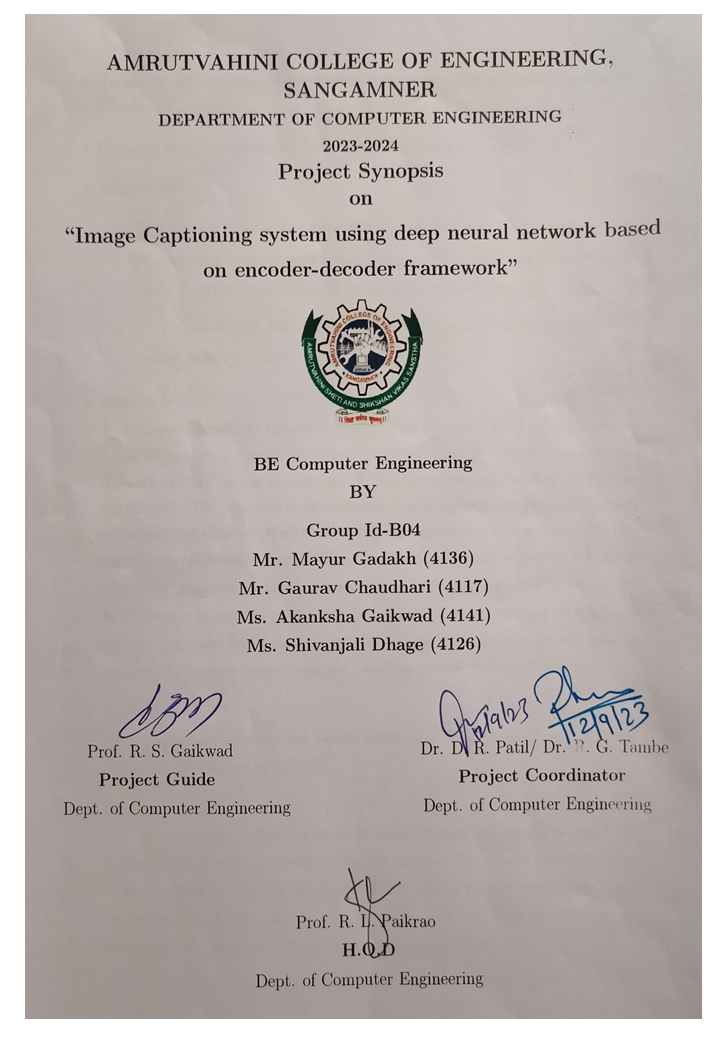
\includegraphics[width=1.010\linewidth]{sys12}
\label{Fig:f4}
\end{center}
\end{figure}

\newpage
\addcontentsline{toc}{chapter}{Abbreviation}
\newpage
{\fontsize{16}{15} \bfseries \LARGE \selectfont \centerline{Abbreviation}}
%{  \newpage {\bfseries \fontsize{14}{12} \selectfont \centerline{Acknowledgment} 
%\vspace*{2\baselineskip}} \setlength{\parindent}{11mm} }
%{ \setlength{\parindent}{0mm} }
\vspace{10mm}

\begin{tabular}{ll}
CNN & Convolutional Neural Network\\ 
RNN  & Recurrent Neural Network\\
GRU & Gated Recurrent Unit\\
LSTM & Long Short Term Memory\\
NLP & Natual Langauage Processing\\
FC & Fully Connected\\
BLEU & BiLingual Evaluation Understudy\\
AI  & Artificial Intelligence\\
VGG-19 & Visual Geometry Group-19\\
CPU & Central Processing Units\\
GPU & Graphical Processing Units\\
TPU & Tensor Processing Units\\
RAM & Random Access Memory\\
NLTK &Natual Language Tool Kit\\
LTS & Long Term Support\\
IDE & Integrated Development Envirnoment\\
SSD & Solid State Drive\\
VM & Virtaul Machine\\
METEOR & Metric for Evaluation of Translation with Explicit ORdering\\
UML & Unified Modeling Language\\

\end{tabular}
\newpage
\addcontentsline{toc}{chapter}{List of Figures}
\newpage

\listoffigures
%{\bf \fontsize{14}{12} \selectfont \centerline{\listoffigures}}
%\listoffigures 

\newpage
\addcontentsline{toc}{chapter}{List of Tables}
\newpage

\listoftables
%{\bf \fontsize{14}{12} \selectfont \centerline{\listoftables}}

% \maketitle
\tableofcontents



\mainmatter



  \titleformat{\chapter}[display]
{\fontsize{16}{15}\filcenter}
{\vspace*{\fill}
 \bfseries\LARGE\MakeUppercase{\chaptertitlename}~\thechapter}
{1pc}
{\bfseries\LARGE\MakeUppercase}
[\thispagestyle{empty}\vspace*{\fill}\newpage]


\setlength{\parindent}{11mm}
\newpage
\cfoot{AVCOE, Department of Computer Engineering 2023-24}

\chapter{Introduction}



The field of computer vision and natural language processing has undergone a remarkable transformation with the emergence of automatic image captioning. This intricate process involves generating concise and contextually relevant textual descriptions for digital images, posing a challenge in discerning crucial objects, understanding their properties and interrelations, and articulating this understanding in coherent linguistic representation. Bridging this semantic gap requires a harmonious fusion of sophisticated computer vision techniques and robust language models derived from Natural Language Processing (NLP).
\\
Traditionally, the synergy of machine learning and NLP has autonomously deciphered the content within images. Deep neural network strategies, notably Convolutional Neural Networks (CNNs) and advanced Recurrent Neural Networks (RNNs) like Long Short-Term Memory (LSTM), have addressed multifaceted challenges associated with image captioning, aiming to provide articulate natural language explanations that capture the essence of depicted scenes.
\\
This study advances the state-of-the-art by proposing an innovative image captioning framework. At its core, the model leverages the robust feature extraction capabilities of ``EfficientNetV2" as the CNN encoder, coupled with the sequential processing prowess of a Gated Recurrent Unit (GRU). Notably, our approach diverges from convention by introducing an attention mechanism tailored for images, enabling the model to selectively focus on specific regions, enriching the contextual depth of generated captions.
\\
While preceding studies have explored diverse methodologies, our proposed model distinguishes itself through the strategic integration of EfficientNetV2 and GRU, coupled with a bespoke attention mechanism. The deliberate choice of the Flickr8k dataset for training and evaluation ensures a focused and cohesive analysis aligned with the intricacies of our model. The conventional encoder-decoder pipeline undergoes a paradigm shift, with EfficientNetV2 pre-trained on the dataset and a GRU serving as a decoder to construct meaningful image descriptions.
\\
In contrast to traditional architectures like CNNs and LSTMs, our approach strategically leverages the unique strengths of EfficientNetV2 and GRU. The project's experimental phase encompasses rigorous training and meticulous testing on the Flickr8k dataset, underpinned by comprehensive performance evaluations utilizing metrics such as BLEU scores. Furthermore, we draw inspiration from related datasets such as MS COCO, Flickr30k, and pertinent local datasets, ensuring a holistic assessment of the proposed image captioning generator.
\\
A Fully Connected (FC) layer, also known as a Dense layer, is a fundamental building block in neural networks. In this layer, each neuron is connected to every neuron in the previous and next layers. These connections are characterized by weights, which are learned during training, and bias terms. The layer computes a weighted sum of its input, adds the bias, and applies an activation function to produce the output. FC layers are crucial for capturing complex relationships in data and are often used in various neural network architectures for tasks like classification and regression.
\\
In the expansive realm of deep learning for image captioning, the synergistic marriage of EfficientNetV2 and Gated Recurrent Unit (GRU) architecture opens up a frontier of possibilities. EfficientNetV2, renowned for its superior efficiency in image feature extraction, seamlessly intertwines with the sequential processing prowess of GRU, creating a holistic model capable of unraveling the intricate narrative within visual content. As we embark on this journey, the aim is to transcend conventional boundaries, pushing the envelope of image captioning capabilities. This exploration not only represents a convergence of cutting-edge technologies but also holds the promise of fostering a deeper, more nuanced comprehension of visual data, ushering in a new era in the symbiotic relationship between deep learning, computer vision, and natural language understanding.


\begin{enumerate}
\item{Image Captioning : }
Image captioning is a computer vision and natural language processing task where a model generates textual descriptions for given images. Utilizing neural networks, particularly encoder-decoder architectures, the model extracts features from the image using an encoder and then decodes these features into a coherent and descriptive sentence. Image captioning combines visual understanding and language generation, making it a multimodal task. This technology finds applications in accessibility tools, aiding visually impaired individuals, and enhances image indexing and retrieval systems. The task involves teaching models to recognize objects, activities, and relationships within images, contributing to a more comprehensive understanding of visual content.
\item {Encoder- decoder Architecture : }
An encoder-decoder model is a neural network architecture designed for sequence-to-sequence tasks. The encoder processes input sequences and compresses them into a fixed-size context or latent representation. The decoder then takes this representation and generates an output sequence step by step. It is commonly employed in tasks such as machine translation, where the input and output sequences can vary in length. The encoder captures the input's semantic information, enabling the decoder to produce meaningful outputs. This architecture is pivotal in natural language processing and image captioning, providing a structured approach to handle sequential data. It facilitates the transfer of information from input to output while accommodating varying lengths of sequences.
\item{EfficientNetV2 : }
At the heart of our image captioning framework lies the EfficientNetV2, a state-of-the-art Convolutional Neural Network (CNN) architecture. EfficientNetV2 is renowned for its efficiency in terms of both computational resources and model parameters while maintaining superior performance in image classification tasks. Developed as an evolution of the EfficientNet architecture, version 2 incorporates novel techniques such as efficient scaling to balance model depth, width, and resolution. Its robust feature extraction capabilities make it an ideal candidate for the initial stage of our image captioning process, enabling the model to grasp salient features within images efficiently.

\item{Gated Recurrent Unit (GRU) : }
Complementing the CNN encoder, our image captioning framework employs a Gated Recurrent Unit (GRU) as the sequential processing component. GRU is a type of Recurrent Neural Network (RNN) that excels in capturing long-term dependencies in sequential data. Unlike traditional RNNs, GRUs feature gating mechanisms that enhance their ability to retain essential information and discard irrelevant details. This makes GRUs well-suited for the task of decoding and generating meaningful natural language descriptions of images based on the features extracted by the CNN encoder.

\item{Teacher Forcing : }
Teacher forcing is a training approach in sequence-to-sequence models. During training, the model is fed true output sequences as input. This accelerates learning by guiding the model with correct sequences. In contrast, during inference, the model generates outputs based on its own predictions, potentially leading to exposure bias. Teacher forcing helps in capturing dependencies between input and output sequences. It is widely used in tasks like language translation and image captioning. The method aids faster convergence during training. However, the model might face challenges during testing due to discrepancies between training and inference conditions. To address this, a combination of teacher forcing and other techniques is often employed.



\item {Attention Mechanism : }
A pivotal innovation in our image captioning framework is the incorporation of an attention mechanism tailored for images. Attention mechanisms have proven invaluable in natural language processing tasks, allowing models to focus on specific parts of input sequences when generating corresponding outputs. In the context of image captioning, our attention mechanism enables the model to selectively attend to relevant regions of the input image during the decoding phase. This adaptive focus enriches the contextual depth of the generated captions, ensuring that the model attends to the most pertinent visual features when constructing textual descriptions.

\end{enumerate}
As the project unfolds, substantial contributions to the field are envisaged. By addressing the limitations of existing models and introducing novel components like EfficientNetV2 and GRU with an attention mechanism, our endeavor strives to set new benchmarks for the performance of automatic image captioning technology. This introduction lays the groundwork for a rigorous exploration into the nuances of image comprehension and caption generation, propelling the field towards enhanced capabilities and broader applicability.
\newpage
\section{Project Idea}
The project endeavors to create an advanced image captioning system, leveraging cutting-edge deep learning techniques, including EfficientNetV2 and GRU. By combining these state-of-the-art models, the system aims to produce rich and contextually relevant textual descriptions for images. This venture sits at the intersection of computer vision and natural language processing, addressing the complex challenge of bridging visual understanding and linguistic expression. With a focus on automation, the system seeks to enhance accessibility for visually impaired individuals and improve image indexing for efficient retrieval. The utilization of EfficientNetV2 ensures robust feature extraction from images, while the GRU facilitates sequential information processing for fluent caption generation. This project contributes to the evolving landscape of multimodal AI systems, fostering a deeper integration of visual and textual understanding. The exploration of EfficientNetV2 and GRU techniques aligns with the forefront of deep learning, promising innovative strides in the field of image captioning.
\section{Motivation of the Project}  
To bridge the gap between computer vision and natural language understanding through the development of an advanced image captioning system, this project is driven by the recognition that seamlessly integrating visual and linguistic capabilities holds immense potential for enhancing various applications in artificial intelligence and deep learning. The emphasis on image captioning stems from its status as a highly valuable skill, presenting substantial opportunities for career growth in the dynamically evolving fields of AI and deep learning. The project's motivation extends beyond technical innovation to address the practical implications of creating systems that can interpret and articulate visual content. By advancing image captioning techniques, the project aims to contribute to the broader landscape of AI applications, empowering individuals and industries with more intuitive and comprehensive tools for image analysis and understanding.


\chapter{Literature Survey}
\section{Literature Survey}
\begin{enumerate}
\item{This study introduces a deep neural network framework for automatic image captioning. It utilizes a Convolutional Neural Network (CNN) encoder to grasp spatial details and recognize objects in images, extracting features for creating a descriptive vocabulary. A Long Short-Term Memory (LSTM) decoder then predicts words and forms coherent sentences. The VGG-19 model serves as an image feature extractor, and the LSTM model processes sequences, producing a fixed-length output vector. The system is trained and tested on various open-source datasets like Flickr 8k, Flickr 30k, and MS COCO using Python, Keras, and TensorFlow. Performance is evaluated using the BLEU metric.}\cite{r1}

\item{Image captioning is evolving as an interesting area of research that involves generating a caption or describing the content in the image automatically. The idea behind image captioning is to make the computer perceive a given image like a human mind leading to automatic description. Image captioning is a challenging task that involves capturing semantically correct information and expressing in a simple sentence. A large number of methods have been proposed in the recent past, and we aim to do a comprehensive survey in the different deep learning algorithms used in image captioning based on the method framework.}\cite{r5}

\item{Image captioning is one of the most recent challenges that caught the interest of the computer vision community as well as the Natural Language Processing community. Recently, the tedious task of image captioning has attained quite notable progress by using numerous techniques. The primary goal of this paper is to study existing Deep Learning techniques for Image Captioning. We have discussed a convolutional neural network-based Image Caption generation model and the salient steps involved in it. We have also discussed dataset and evaluation metrics widely used in fundamental systems.}\cite{r3}


\item{This research explores machine learning algorithms for image and natural language processing, integrating existing packages. It implements an algorithm generating comprehensive sentences from images. After requirements analysis, a bibliographic study informed model selection. A composite model, employing transfer learning in a deep convolutional neural network for feature extraction and a recurrent neural network for descriptions, was designed using Keras with TensorFlow. The result is a trained model capable of describing images in natural language.}\cite{r2}

\item{  Image captioning is a process of automatically describing an image with one or more natural language sentences. In recent years, image captioning has witnessed rapid progress, from initial template-based models to the current ones, based on deep neural networks. This paper gives an overview of issues and recent image captioning research, with a particular emphasis on models that use the deep encoder-decoder architecture. We discuss the advantages and disadvantages of different approaches, along with reviewing some of the most commonly used evaluation metrics and datasets.}\cite{r4}

\end{enumerate}
 

\begin{table}[!htbp]
\begin{center}
\def\arraystretch{1.5}
  \begin{tabular}{| c | c | c | c |}
\hline
Sr. No. &	Paper Title &	Year of & Method \\
&	 &	Publication & Algorithm Used \\

\hline
1 &	Implementing Deep Neural Network  &	 2022  &CNN and RNN \\
 &	 Based Encoder-Decoder Framework    &	 & \\
 &	 for Image Captioning  & 	 &\\
 
\hline
2&Comprehensive Comparative Study on 	  &2022	   &CNN and RNN\\
 & Several Image Captioning Techniques  	  &	 & \\
 &  Based on Deep Learning Algorithm &&\\

 

\hline
3 &An empirical study of image 	  &2021	   &RNN or Transformers\\
 &captioning using deep learning	  &	 &  \\
\hline

\hline
4&	Deep Learning Techniques for  &	 2020 &CNN and RNN \\
 &	Automated Image Captioning &	 & \\
\hline
5&An overview of image caption  	  &2019   &CNN\\
 &generation methods	  &	 & \\
\hline


\end{tabular}
 \caption { Comparative Analysis }
 \label{tab:CompAna}
\end{center}

\end{table}


\chapter{Problem Definition and Scope}
\section{Problem Statement}
Implementing Deep Neural Network Based Encoder-Decoder Framework for Image Captioning using EfficientNetV2 as encoder and GRU as decoder.


\subsection{Goals and objectives}  
Goal and Objectives: 
\begin{itemize}
  	\item To study the deep learning techniques like CNN and RNN.
  	\item To develop a deep-learning based image caption generator that can accurately describe the contents of an image in natural language.
  	\item To create a user-friendly interface for interacting with the image captioning system.
\end{itemize}

 \subsection{Statement of scope} 
	\begin{itemize}  
	\item	Automatic image captioning using deep neural network encoder-decoder frameworks has extensive potential.
\item It can enhance accessibility, content indexing, e-commerce, healthcare, education, and more by generating descriptive image captions.
\item This technology streamlines processes, improves user experiences, and finds applications across diverse domains.
	\end{itemize}

\section{Software context} 
\begin{itemize}
\item The project will involve the development of software components for image captioning using EfficientNetV2 and GRU.
\item The software will include modules for image feature extraction, natural language processing, and model integration.
\item Additionally, the project will utilize relevant libraries, frameworks, and tools for deep learning, image processing, and natural language generation.
\end{itemize}
\section{Major Constraints}
\begin{itemize}
\item \textbf{Computational Resources :} Limited computational power and hardware may impact the speed and scalability of the model training and image caption generation processes, especially when dealing with large datasets like Flickr8k.
\item\textbf{ Data Availability :} In Flickr8k dataset the quality and diversity of these datasets may still pose challenges in terms of data preprocessing, management, and ensuring they are suitable for your specific deep learning models.
\item \textbf{Time Frame :} Meeting project deadlines within the academic semester, while working with multiple datasets and conducting rigorous evaluations, is a crucial constraint, as it may affect the extent of research, development, and testing possible.
\end{itemize}

\section{Methodologies of Problem solving and efficiency issues}
\subsection{Methodologies of Problem Solving}
\begin{itemize}

	\item\textbf{ Feature Extraction with EfficientNetV2 :} Utilize EfficientNetV2 as a feature extractor to represent images effectively. This methodology involves fine-tuning the pre-trained model's layers and extracting high-level features from the images.
	\item \textbf{Caption Generation with GRU :} Implement a GRU-based sequence-to-sequence model for generating captions. This methodology includes training the model to learn the language structure and generate coherent and contextually relevant descriptions.
	\item\textbf{ Data Augmentation :} Apply data augmentation techniques to enhance dataset diversity and reduce overfitting. This involves techniques like image cropping, flipping, and color jittering to improve model generalization.
\end{itemize}
\subsection{ Efficiency Issues}
\begin{itemize}
\item \textbf{Computational Resources :} Address efficiency issues by optimizing model architecture and training procedures to make the best use of available hardware. This includes considering batch sizes, model parallelization, and hardware acceleration (e.g., GPUs).
\item \textbf{Memory Management : }Efficiently manage memory during training and inference to handle large datasets and avoid memory bottlenecks. Techniques such as batch loading, memory-efficient data structures, and model quantization can be explored.

\item \textbf{Real-time Inference :} Optimize the caption generation process for real-time applications by improving model inference speed. This can involve quantization, model compression, and deployment on hardware suitable for real-time processing.
\end{itemize}

\section{Scenario in which multi-core, Embedded and Distributed Computing used}
\begin{itemize}
\item\textbf{ Multi-Core Utilization :} Leveraging multi-core processing is essential for parallelizing image processing tasks, enabling simultaneous feature extraction and caption generation for multiple images. This approach optimizes computational efficiency, reducing the time taken to process large volumes of images and generate captions.

\item \textbf{Embedded Computing :} Implementing the image captioning system on embedded devices, such as edge computing platforms and IoT devices, allows for on-device processing without relying heavily on external computing resources. This approach ensures the availability of real-time captioning capabilities in applications where network connectivity may be limited or unstable.
\item \textbf{Distributed Computing :} Utilizing distributed computing allows the system to distribute computational tasks across multiple nodes, optimizing the processing of extensive datasets and complex neural network models. By utilizing a distributed architecture, the image captioning system can handle large-scale image processing and caption generation, catering to the demands of high-throughput applications.
\end{itemize}


\section{Outcome}
The outcomes of implementing image captioning using EfficientNetV2 and GRU are multifaceted:
\begin{itemize}

\item \textbf{Enhanced Accessibility :} It makes visual content more accessible to individuals with visual impairments, as it provides descriptions for images, enabling a richer online experience.

\item \textbf{Automated Tagging :} The technology automates the process of tagging and categorizing images, which can significantly improve content organization and retrieval.

\item \textbf{Content Recommendation :} It enables more intelligent content recommendation systems by understanding the visual content of images and associating them with user preferences.

\item \textbf{Improved Human-Computer Interaction :} The ability to generate captions for images enhances human-computer interactions, making it easier for users to interact with and search for visual content.

\item \textbf{Advancements in AI :} It exemplifies the progress in AI and deep learning, showcasing how neural networks can bridge the gap between visual and textual information.

\end{itemize}

\section{Applications}
\begin{itemize}
\item \textbf{Social Media : }Image captioning is commonly used on social media platforms to automatically generate captions for user-uploaded images, making content more engaging and informative.
 \item \textbf{Content Recommendation : }Image captions can be used to personalize content recommendations by analyzing the textual descriptions and user preferences, improving user engagement and retention.
 \item \textbf{E-commerce : }Image captioning can provide product descriptions and details for e-commerce websites, enhancing the shopping experience by offering detailed information about products.
 \item \textbf{Education : }Image captioning can be applied in educational materials to provide additional context and information for images in textbooks, online courses, and educational websites.
\end{itemize}

\section{Hardware Resources Required}
\begin{table}[!htbp]
\begin{center}
\def\arraystretch{1.5}
  \begin{tabular}{| c | c | c | c |}
\hline
Sr. No. &	Parameter &	Minimum  & Justification \\
&&Requirement&\\
\hline
1 &	CPU Speed &	 2 GHz  & Required for efficient processing\\
&&& of image data \\
\hline
2 &	RAM  &	8 GB &  Necessary for handling the computational \\
&&& load during  image captioning\\
\hline
3 & GPU & 2 GB & Required for fast processing \\
 \hline
\end{tabular}
 \caption { Hardware Requirements }
 \label{tab:hreq}
\end{center}

\end{table}


\section{Software Resources Required}
Platform : 
\begin{enumerate}
\item Operating System : Windows 10 or Ubuntu 20.04 LTS
\item IDE : PyCharm or Jupyter Notebook
\item Programming Language : Python 3.7 or higher, with libraries such as TensorFlow, NLTK, and NumPy.
\end{enumerate}

\chapter{Software Requirement Specification  }
\section{Introduction}
\subsection{Purpose and Scope of Document}
The purpose of this document is to outline the design and implementation of a Deep Neural Network-based Encoder-Decoder framework for Image Captioning. This framework combines Convolutional Neural Networks (CNNs) to encode images and Recurrent Neural Networks (RNNs) to generate descriptive captions. \\The scope includes explaining the architecture, training process, and evaluation metrics for image captioning tasks. It provides a comprehensive guide for researchers and developers interested in creating image captioning systems, enabling them to understand the key components, techniques, and considerations involved in this field. The document aims to bridge the gap between theory and practical implementation in the domain of computer vision and natural language processing.

\subsection{Overview of responsibilities of Developer}
The developer's responsibilities in implementing a Deep Neural Network-based Encoder-Decoder framework for Image Captioning include
\begin{itemize}


\item \textbf{Data Preprocessing :} Collect, clean, and preprocess image and caption data, ensuring it's suitable for training the model.

\item \textbf{Architecture Design :} Design the neural network architecture, combining CNNs and RNNs, specifying the number of layers, units, and activation functions.

\item \textbf{Model Implementation : }Code the framework using deep learning libraries (e.g., TensorFlow, PyTorch) and integrate the encoder-decoder structure.

\item \textbf{Hyperparameter Tuning : }Optimize hyperparameters like learning rates, batch sizes, and sequence lengths for better model performance.

\item \textbf{Training :} Train the model on the prepared dataset, monitoring loss and performance metrics.
\end{itemize}
  
\section{Functional Requirements}
  
 \subsection{System Feature 1 (Image Preprocessing Module)}  
The system must have a module for preprocessing input images to make them suitable for the image captioning model. The image preprocessing module in image captioning prepares raw images for analysis by resizing, normalizing pixel values, and potentially augmenting data. It enhances feature extraction by ensuring consistent image dimensions and colour ranges, facilitating subsequent deep learning model input. This module improves model performance and consistency in generating accurate image captions.


\subsection{System Feature 2 (Encoder-Decoder Architecture)}
The core of the system is the Encoder-Decoder architecture, where the image is encoded using a Convolutional Neural Network (CNN) and the encoded information is decoded into a caption using a Recurrent Neural Network (RNN).The Encoder-Decoder architecture is a fundamental framework used in image captioning. The encoder processes the input image, typically using convolutional neural networks (CNNs) to extract image features. The decoder, often using recurrent neural networks (RNNs) or transformer models, generates a textual caption based on the extracted features. This approach combines computer vision and natural language processing to produce coherent and contextually relevant image captions. \\ 
This feature includes:
\begin{itemize}
\item \textbf{Image Encoding :} The system implements the EfficientNetV2 model to effectively encode images, enabling comprehensive feature extraction and representation from input images for subsequent processing in the caption generation process.
\item \textbf{Caption Generation : } The system utilizes the GRU (Gated Recurrent Unit) model for generating natural language captions from the encoded image information. This process involves leveraging the GRU's sequential processing capability to produce coherent and contextually relevant captions for the provided images.
\item \textbf{Connection Between Encoder and Decoder : }The system establishes an efficient connection between the image encoder, implemented with EfficientNetV2, and the caption decoder, implemented with GRU. This integration ensures smooth information flow from the encoded image representation to the caption generation module, facilitating a seamless and accurate translation of visual features into descriptive captions.
\end{itemize}

\subsection{System Feature 3 (Model Training and Fine-Tuning)}
 This feature involves the training and fine-tuning of the neural network model to ensure it can effectively generate accurate and contextually relevant image captions. \\It includes the following components:
\begin{itemize}
\item \textbf{Training Data :} The system employs diverse dataset, including Flickr8k to train the neural network model. This comprehensive training data helps the model gain a robust understanding of various visual contexts and linguistic patterns, enabling it to generate accurate and contextually relevant captions.
\item \textbf{Loss function :} The system incorporates a customized loss function tailored to the specific requirements of the EfficientNetV2 and GRU-based architecture. This specialized loss function optimizes the model's training process, ensuring efficient fine-tuning and improved caption generation performance.
\end{itemize}
These components collectively contribute to the effective training and fine-tuning of the neural network model, enhancing its capability to generate accurate and contextually relevant image captions.


\section{External Interface Requirements (If Any)}
\subsection{User Interfaces}
\begin{itemize}
\item \textbf{Image Upload/Selection : }Allow users to upload or select images for captioning. You can include an option for capturing images from a camera.
\item \textbf{Caption Display :} Display the generated image captions in a clear and readable format.
\item\textbf{ Caption Customization :} Provide options for users to customize the generated captions, such as adjusting length, style, or language.
\item \textbf{Caption Generation Button :} Include a button or action to trigger the caption generation process.
\item \textbf{Image Preview :} Show a preview of the uploaded image(s) to confirm the selection.
\item \textbf{Accessibility Features : }Make the interface accessible to users with disabilities, including alt text for images and keyboard navigation.
\item\textbf{ Error Handling : }Implement error messages and guidance for users in case of issues with image processing or caption generation.
\item \textbf{Privacy and Security : }Clearly communicate how user data and images are handled and stored, addressing privacy and security concerns.


\end{itemize}


\subsection{Hardware Interfaces}
\begin{itemize}
\item \textbf{Input Devices :} For non-real-time or batch processing, users can upload images from various sources, including:
Computer storage (hard drive, SSD)
External storage devices (USB drives, SD cards)
\item \textbf{Processing Unit (CPU/GPU) :} The image captioning model requires significant computational power for image analysis and caption generation. A CPU and/or GPU is used for this purpose. Modern deep learning models benefit greatly from GPUs due to their parallel processing capabilities.
\item \textbf{Memory (RAM) : }Sufficient RAM is essential for loading and processing images, especially when dealing with large datasets or multiple concurrent users.
\item \textbf{Storage :} The system should have storage capacity for storing images, model parameters, and generated captions. SSDs or large-capacity hard drives are common choices.
\item \textbf{Network Interface :} A network connection is necessary for accessing image databases, model updates, and potentially sharing or storing captioned images online.
\item \textbf{Display :} A monitor or screen is needed to display the user interface and the captioned images. It can be a desktop monitor, laptop screen, or the screen of a mobile device.
\item \textbf{Peripheral Devices :} Input devices such as keyboards, mice, and touchscreens are necessary for user interaction with the system.


\end{itemize}
\subsection{Software Interfaces}
\begin{itemize}
\item \textbf{Image Input :}
Allow users to upload or provide images for captioning. You can use file upload widgets or device cameras (for mobile apps).
\item \textbf{Image Processing :}
Preprocess the input image. This may involve resizing, normalizing, and enhancing the image to improve model performance.
\item \textbf{Caption Generation :}
Pass the image features through the NLP model to generate captions for the image. These captions can be single sentences or multiple sentences depending on the complexity of the image.


\end{itemize}
\section{Nonfunctional Requirements}  
\subsection{Performance Requirements} 
Performance requirements for an image captioning project using deep learning are critical to ensure that the system meets user expectations and operates efficiently. Here are key performance requirements to consider:
\begin{itemize}


\item \textbf{Accuracy : }The image captioning model should provide accurate and meaningful captions for a wide range of images. Define a minimum accuracy threshold, such as BLEU, METEOR, or CIDEr scores, to evaluate model performance.
\item \textbf{Speed : }Define the expected response time for generating captions. Users generally expect quick results, so set a maximum response time to meet user experience expectations.
\item \textbf{Scalability : }Ensure that the system can handle an increasing number of users and images. Define performance requirements for both horizontal (adding more servers) and vertical (scaling a single server) scalability.
\item \textbf{Latency : }Define maximum acceptable response times for generating captions for different image sizes. Ensure low-latency interactions with the user interface.
\end{itemize}
\subsection{Safety Requirements}
\begin{itemize}
\item \textbf{Privacy Protection : }Ensure that user data and uploaded images are protected and not shared with unauthorized parties. Comply with data protection regulations such as GDPR or HIPAA, as applicable.
\item \textbf{Transparency and Explainability : }Make the image captioning process as transparent and explainable as possible. Users should understand how captions are generated, and there should be a way to provide explanations for generated captions when requested.

\end{itemize}


\subsection{Security Requirements }
\begin{itemize}
\item \textbf{Data Encryption :}
Implement data encryption in transit (using HTTPS) and at rest to protect image data and captions from unauthorized access or interception.
\item \textbf{Secure Data Storage :}
Ensure that user data and uploaded images are securely stored with appropriate access controls to prevent unauthorized access.


\end{itemize}
\subsection{Software Quality Attributes }
\begin{itemize}
\item \textbf{Accuracy :}
The accuracy of generated captions is crucial. Captions should closely match the content of the images.

\item \textbf{Performance :}
The system should generate captions quickly, especially for real-time or interactive applications.

\item \textbf{Scalability :}
The ability to handle a growing number of users and images without significant degradation in performance is essential.

\item \textbf{Usability :}
The user interface should be intuitive and user-friendly, making it easy for users to interact with the system.

\item \textbf{Security :}
User data and generated captions should be protected from unauthorized access and breaches.

\item \textbf{Maintainability :}
The codebase should be well-structured, documented, and easy to maintain, allowing for updates and improvements.

\item \textbf{Reliability :}
The system should be available and responsive, with minimal downtime.

\end{itemize}
\section{System  Requirements }  
 
\subsection{Database Requirements}  
To implement image captioning, we select a dataset flickr8k in which 8k images and 8k captions included.

\subsection{Software Resources Required}
Platform : 
\begin{enumerate}
\item Operating System : Windows 10 or Ubuntu 20.04 LTS
\item IDE : PyCharm or Jupyter Notebook
\item Programming Language : Python 3.7 or higher, with libraries such as TensorFlow, NLTK, and NumPy.
\end{enumerate}

\subsection{Hardware Resources Required}
\begin{enumerate}
\item{CPU : Speed 2 GHz Required for efficient processing of image data.}
\item{RAM : 8 GB Necessary for handling the computational load during image captioning.}
\item{GPU : Minimum 2 GB dedicated GPU is required for less training \& testing time.}

\end{enumerate}
 
\section{Analysis Models: SDLC Model to be applied}

\begin{figure}[H]
\begin{center}
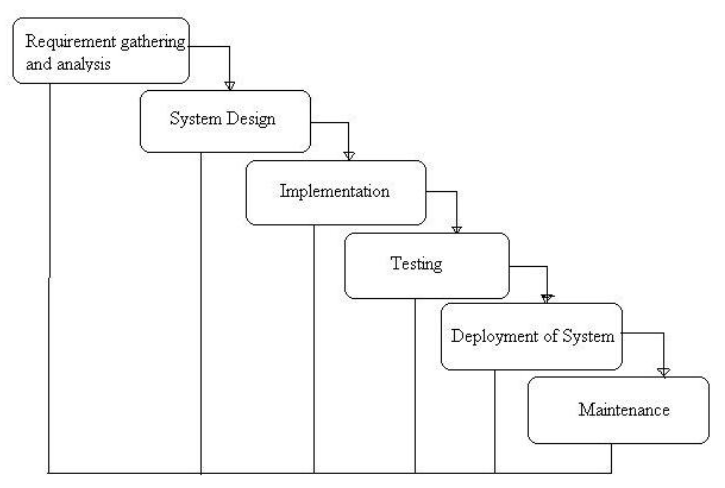
\includegraphics[width=1.0\linewidth]{waterfall}
\caption*{}
\label{Fig:f1}
\end{center}
\end{figure} 
The Waterfall Model is a traditional software development methodology that follows a linear and sequential approach, consisting of distinct phases such as requirements, design, implementation, testing, and maintenance. While the Waterfall Model is more commonly associated with traditional software development, it is not typically used for deep learning tasks like image captioning, which involve a more iterative and experimental process. Deep learning models are often developed using iterative approaches, where the model is trained, evaluated, and refined in multiple cycles.\\
The application of the waterfall model to image captioning using deep learning, specifically with EfficientNetV2 and Gated Recurrent Unit (GRU), provides a structured and sequential approach. The cascade of processes, from feature extraction with EfficientNetV2 to context modeling with GRU, exemplifies a systematic flow in the development lifecycle. This methodology ensures a step-by-step refinement, allowing for a thorough exploration of the interplay between visual and textual information. As we conclude this endeavor, the waterfall model's rigidity aligns with the meticulous integration of EfficientNetV2 and GRU, contributing to a comprehensive and well-defined framework for advancing image captioning capabilities within the realm of deep learning.\\
The process can be described as follows:

\begin{itemize}


\item{\textbf{Requirements :  }}
Define the requirements for the image captioning system, including input data specifications, desired captioning output, and performance metrics.
\item{\textbf{Design : }}
Design the architecture of the deep learning model, including specifying the type of neural network (e.g., CNN-RNN), deciding on model parameters, and planning data preprocessing steps.
\item{\textbf{Implementation : }}
Develop and implement the deep learning model according to the designed architecture using a framework like TensorFlow or PyTorch.
\item{\textbf{Testing : }}
Evaluate the model on a validation dataset to assess its performance. This involves measuring metrics such as accuracy, BLEU scores, or other evaluation criteria relevant to image captioning.
\item{\textbf{Deployment : }}
If the model meets the desired performance criteria, deploy it for real-world use. This may involve integrating the model into an application or system capable of accepting input images and generating captions.
\item{\textbf{Maintenance : }}
Periodically update and fine-tune the model based on new data or changing requirements. Maintenance may also involve addressing issues discovered during real-world usage.

\end{itemize}

\section{System Implementation Plan :}
\begin{figure}[H]
\begin{center}
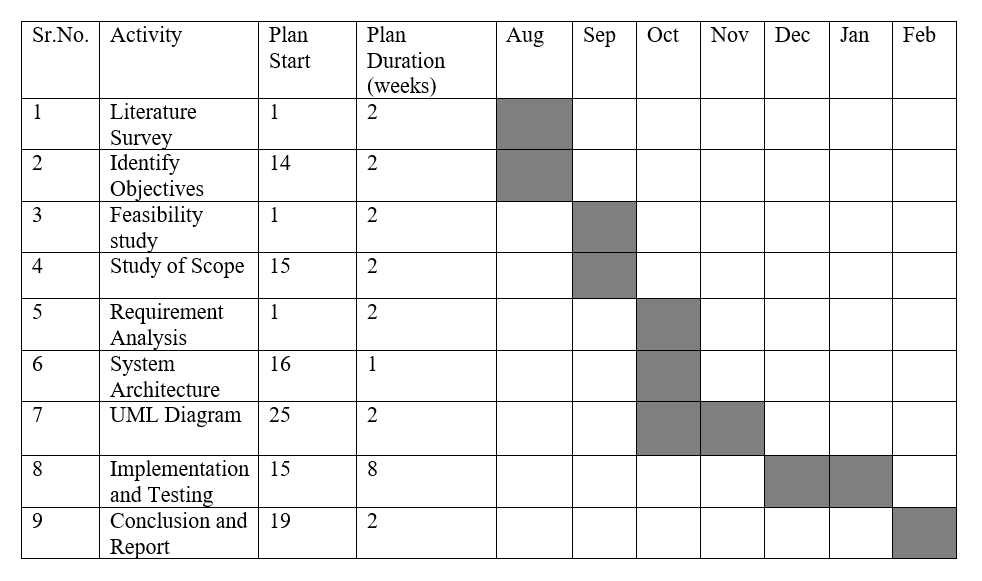
\includegraphics[width=1.0\linewidth]{sys34}
\caption{System Implementation}
\label{Fig:f2}
\end{center}
\end{figure}



\chapter{Methodology and System Design}


\section{System Architecture}  
\begin{figure}[H]
\begin{center}
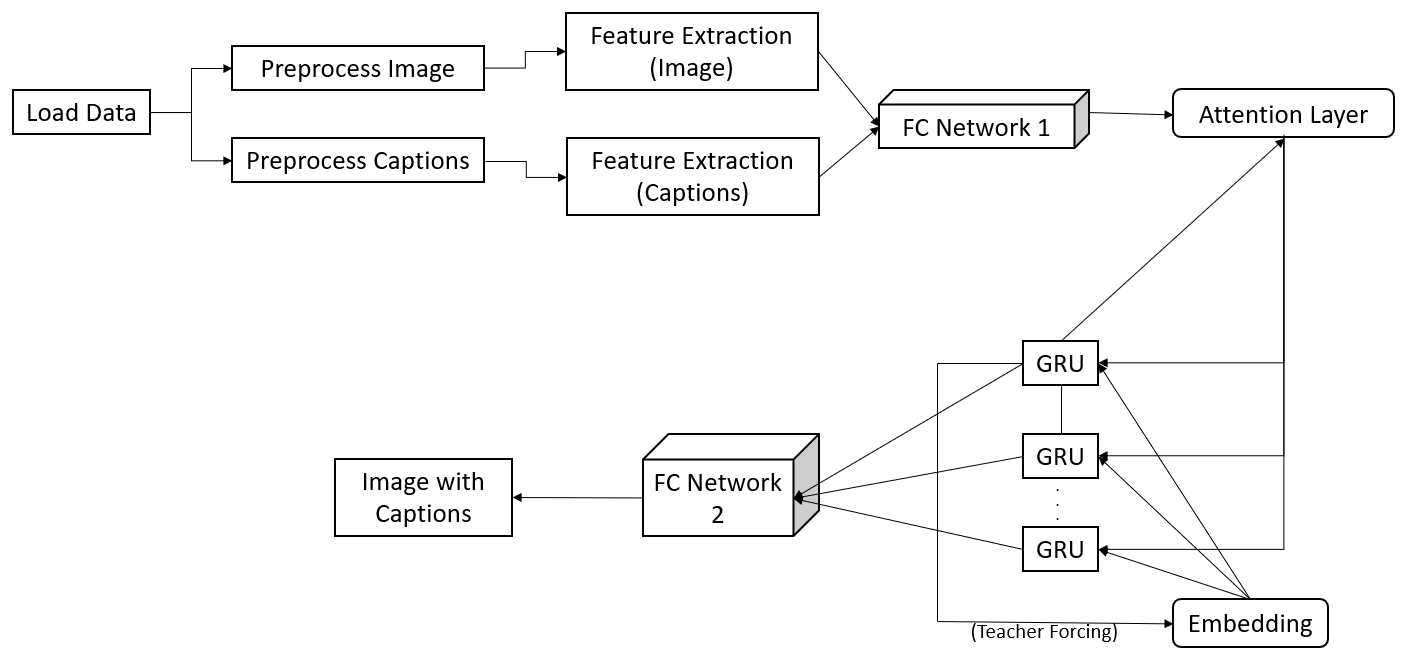
\includegraphics[width=1.0\linewidth]{sysff}
\caption{System Architecture}
\label{Fig:f1}
\end{center}
\end{figure}
The image caption generation system begins with the pivotal step of loading data, encompassing a curated dataset of images and their corresponding captions. Subsequently, meticulous data preparation unfolds, involving resizing images, normalizing pixel values, and tokenizing captions for streamlined processing. The heart of the architecture lies in feature extraction, where Convolutional Neural Networks (CNNs) like EfficientNetV2 are employed to distill high-level visual features from the images. These extracted features serve as inputs for the image caption generation model, typically implemented using GRU. During the training phase, the model refines its parameters by predicting the next word in a sequence, learning the intricate associations between visual context and generated captions. The training data, consisting of image-caption pairs, fuels this iterative learning process through optimization algorithms like stochastic gradient descent. The integrated system encompasses components for user input, caption generation, and potential post-processing, culminating in a deployment-ready architecture that can generate descriptive captions for input images in real-world scenarios.
This holistic architecture, combining EfficientNetV2, GRU, teacher forcing, and attention mechanisms, forms a sophisticated system for image captioning. It not only leverages the efficiency of EfficientNetV2 in visual feature extraction but also benefits from the sequential modeling capabilities of GRU, enhanced by attention mechanisms. 

\section{Data Flow Diagrams}  
\begin{figure}[H]
\begin{center}
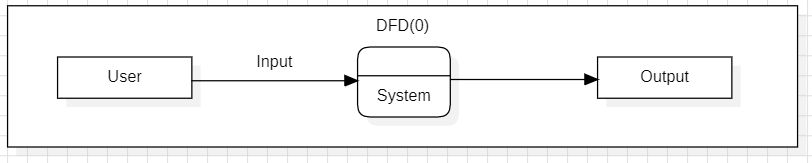
\includegraphics[width=1.0\linewidth]{dfd0}
\caption{DFD0}
\label{Fig:f2}
\end{center}
\end{figure}
  
\begin{figure}[H]
\begin{center}
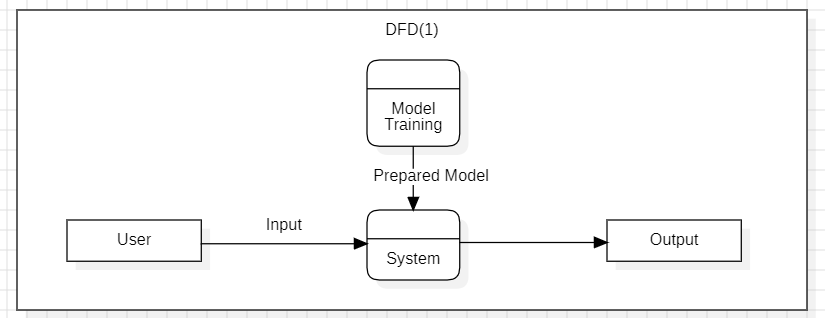
\includegraphics[width=1.0\linewidth]{dfd11}
\caption{DFD1}
\label{Fig:f2}
\end{center}
\end{figure}
  
\begin{figure}[H]
\begin{center}
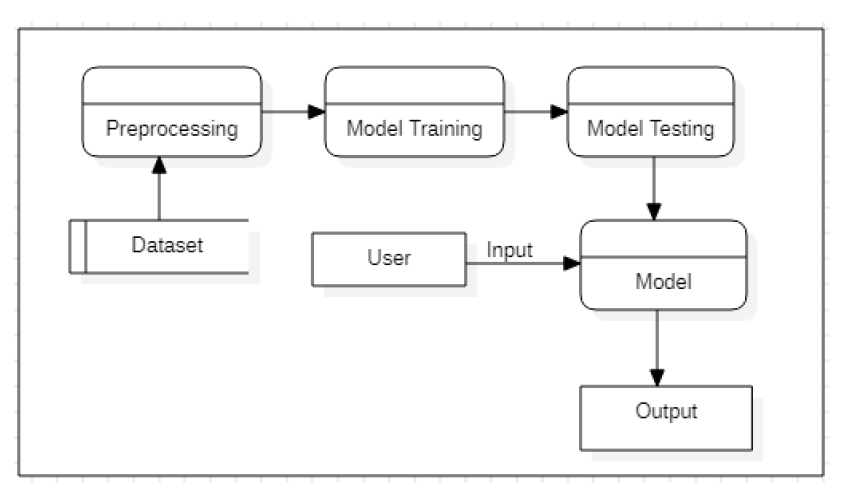
\includegraphics[width=1.0\linewidth]{dfd2}
\caption{DFD2}
\label{Fig:f2}
\end{center}
\end{figure}

A Data Flow Diagram (DFD) visually represents the flow of data within a system.\\
\begin{itemize}


\item{External Entities : }
User: Initiates the image captioning process by uploading an image.
\item{Upload and Preprocess Image : }
Accepts the uploaded image from the user.
Performs data preprocessing on the image (resizing, normalization, etc.).Outputs the preprocessed image data.
\item{Feature Extraction : }
Takes the preprocessed image data as input.Utilizes a feature extraction model (e.g., EfficientNetV2) to extract relevant features.Outputs the extracted features.
\item{Generate Caption : }
Takes the extracted features as input.Utilizes a caption generation model (e.g., GRU with attention) to generate captions.
\item {Display Image and Caption : }
Presents the original image and the generated caption to the user.

\item{Image Database : }
Stores information about images, including ImageID, FilePath, Timestamp.
\item{Caption Database : }
Stores generated captions, including CaptionID, CaptionText, Timestamp.This DFD provides an overview of the processes involved in image captioning, including data inputs, transformations, and outputs.

\end{itemize}
The system involves a user initiating image captioning by uploading an image, which undergoes preprocessing and is fed into a feature extraction model (e.g., EfficientNetV2). Extracted features are then used in a caption generation model (e.g., GRU with attention) to produce captions. The original image and generated caption are displayed to the user. Information about images is stored in an Image Database, and generated captions are stored in a Caption Database, both with timestamps for reference and organization. This integrated process provides a comprehensive framework for image captioning, encompassing user interaction, data processing, feature extraction, caption generation, and result presentation.
\section{Entity Relationship Diagrams}   
\begin{figure}[H]
\begin{center}
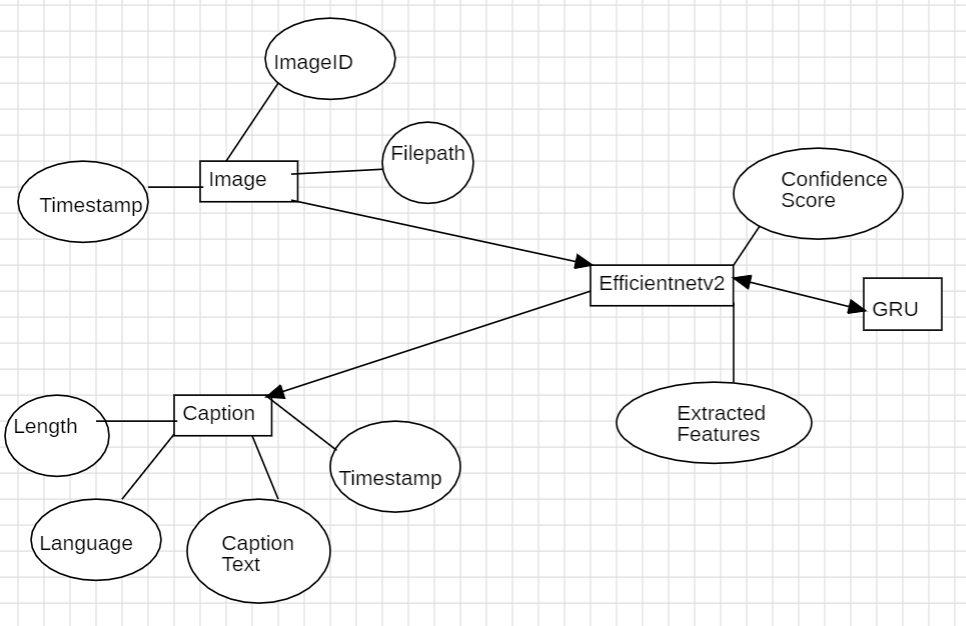
\includegraphics[width=1.0\linewidth]{er1}
\caption{Entity Relationship Diagrams}
\label{Fig:f3}
\end{center}
\end{figure}
An Entity-Relationship (ER) diagram typically represents the entities and relationships in a database. In image captioning with deep learning, the entities include caption, Image, EfficientNetV2 and GRU.
The Entity-Relationship Diagram (ERD) illustrates the interconnected entities in the image captioning system. The ``Image" entity encompasses attributes such as ImageID, FilePath, and Timestamp, forming a one-to-many relationship with the ``Caption" entity, which consists of CaptionID, CaptionText, and Timestamp. Both entities are associated with the ``EfficientNetV2" and ``GRU" entities, representing many-to-one relationships, as multiple images share the same feature extraction and caption generation models. The ``EfficientNetV2" entity includes ModelID, Architecture, and Parameters, while the ``GRU" entity encompasses ModelID, Architecture, Attention, and Parameters. This structured ERD encapsulates the integral components, relationships, and attributes within the image captioning system, providing a comprehensive overview of its architecture and data flow.
\section{UML Diagrams} 
\subsection{Use Case Diagram}
\begin{figure}[H]
\begin{center}
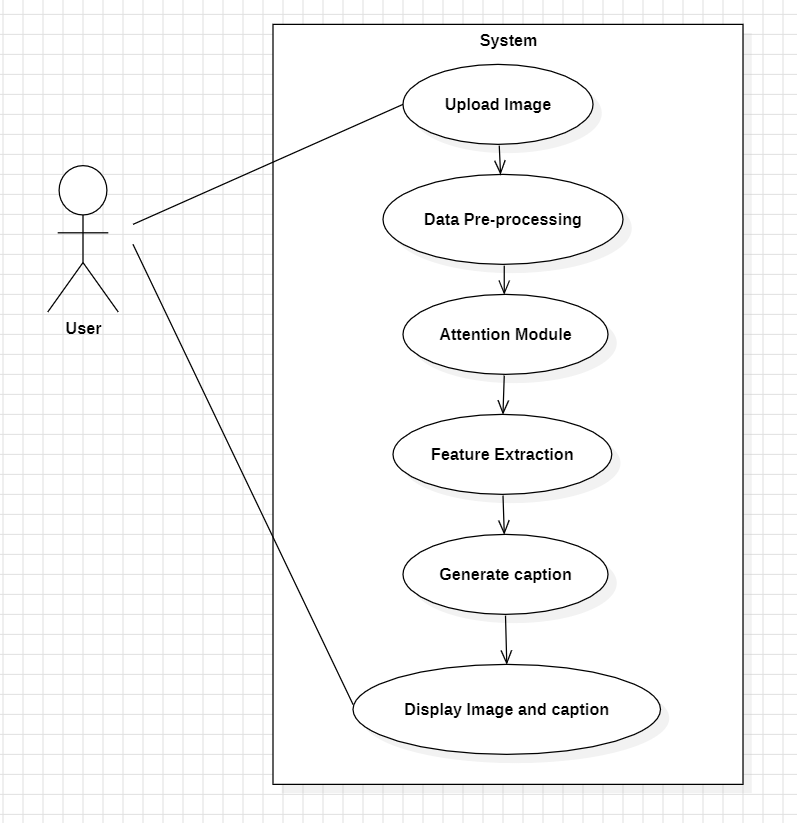
\includegraphics[width=1.0\linewidth]{us1}
\caption{Use Case Diagram}

\label{Fig:f4}
\end{center}
\end{figure}

A use case diagram for image captioning provides a high-level view of the system's functionalities and interactions with external actors. The actor represent entities that interact with the system, and use cases represent specific functionalities or features provided by the system. Here's a simplified use case diagram for an image captioning system.\cite{r6}

\subsection{Activity Diagram}
\begin{figure}[H]
\begin{center}
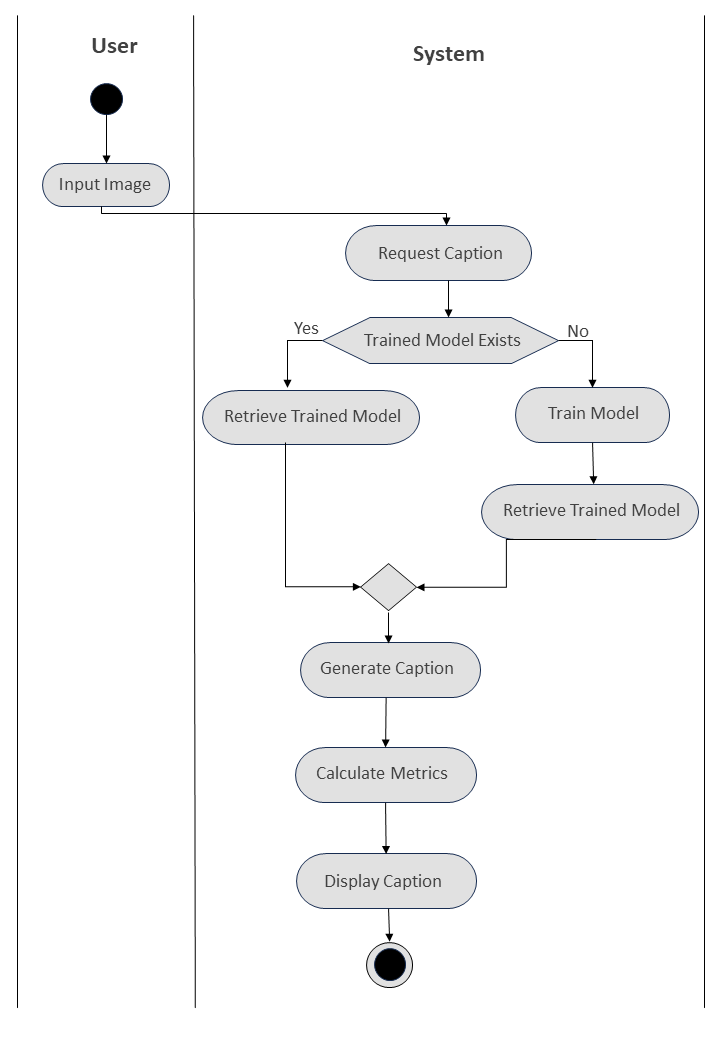
\includegraphics[width=1.0\linewidth]{ac}
\caption{Activity Diagram}
\label{Fig:f4}
\end{center}
\end{figure}

\begin{itemize}


\item An activity diagram for image captioning can illustrate the flow of activities involved in the process.
\item ``Image User" is an actor representing the user interacting with the system.
\item{``Upload Image" is a use case where the user uploads an image for captioning.}
\item{``Image Captioning System" is a use case representing the overall image captioning process.}
\item{``Receive Caption and Display" is a use case where the system receives the generated caption and displays it to the user.}
\item{``Generate Caption for Image" is a use case responsible for actually generating the caption for the uploaded image.}
\item{The ``Image User" actor interacts with the system through ``Upload Image" and receives the caption through ``Receive Caption and Display."}
\item{This diagram illustrates the high-level interactions and functionalities involved in the image captioning The ``Image User" actor starts by uploading an image.}
\item{The ``Captioning Requester" initiates the request for a caption.}
\item{The ``Image Captioning System" generates a caption for the uploaded image.}
\item{The ``Metrics Calculation System" calculates metrics for the generated caption.}
\item{Arrows indicate the flow of activities, and each box represents an activity or a system component.}
\item{This diagram provides a visual representation of the sequential steps involved in the image captioning process, including uploading an image, requesting a caption, generating the caption, and calculating metrics for evaluation.}
\end{itemize}

\subsection{Sequence Diagram}
\begin{figure}[H]
\begin{center}
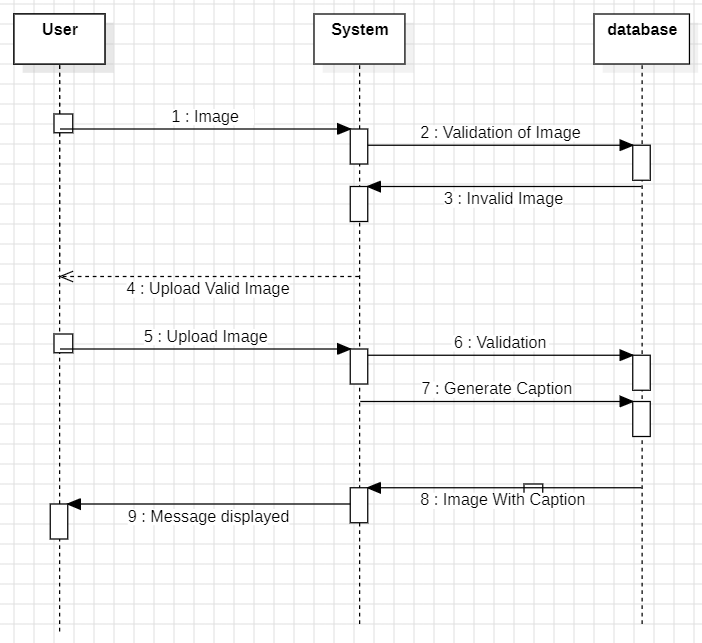
\includegraphics[width=1.0\linewidth]{sequence}
\caption{Sequence Diagram}
\label{Fig:f4}
\end{center}
\end{figure}
\begin{itemize}
\item A sequence diagram for image captioning can help illustrate the interactions between different components or objects in a chronological order.
\item In this sequence diagram:
\item The ``Image User" uploads an image.
\item The ``Image Validation" component validates the uploaded image.
\item If the image is valid, it is uploaded to the ``Image Captioning System."
\item The ``Image Captioning System" generates a caption for the image.
\item The final result is an ``Image with Caption."
\end{itemize}




\subsection{Class Diagram}


\begin{figure}[H]
\begin{center}
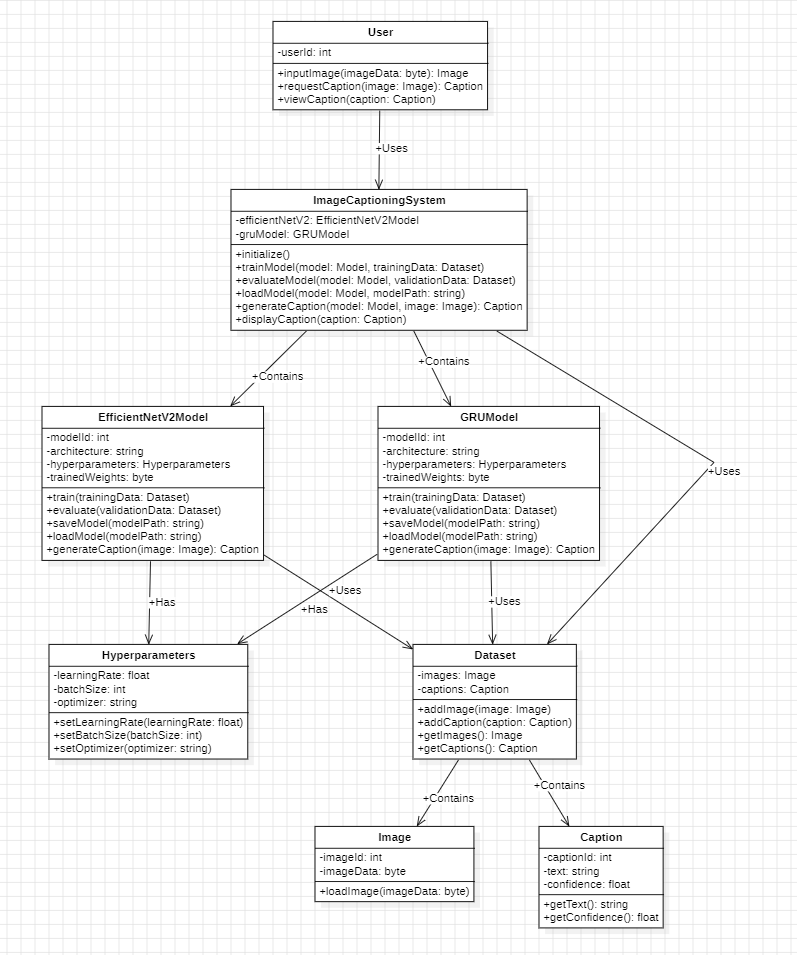
\includegraphics[width=1.0\linewidth]{class1}
\caption{Class Diagram}
\label{Fig:f4}
\end{center}
\end{figure}
In a class diagram for image captioning with deep learning, you can represent classes, their attributes, and methods. The central class in this system is the ImageCaptioningSystem, which encapsulates the entire image captioning functionality. It is associated with two main components: the ImageProcessor and the CaptionGenerator. The ImageProcessor class is responsible for handling image-related operations.\cite{r6}
\subsection{Object Diagram}

\begin{figure}[H]
\begin{center}
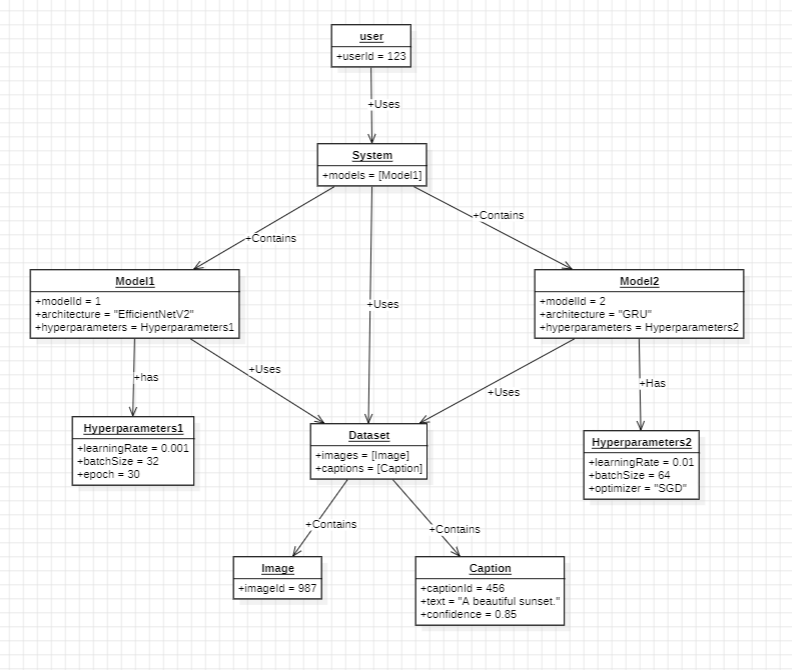
\includegraphics[width=1.0\linewidth]{objf}
\caption{Object Diagram}
\label{Fig:f4}
\end{center}
\end{figure}
An object diagram illustrates instances of classes and their relationships at a specific point in time. In the context of image captioning with deep learning, we have instances of the classes mentioned in the class diagram. imageCaptionSystemInstance contains a composition relationship with imageProcessorInstance, indicating that the ImageProcessor is a vital part of the ImageCaptioningSystem. It also has an association with captionGeneratorInstance. imageProcessorInstance is associated with imageInstance, showcasing that it processes this particular image. The instances of various classes represent the specific components involved in image captioning. The relationships and associations illustrate how these instances collaborate within the system\cite{r6}




\chapter{Software Implementation}
\section{TECHNOLOGY DETAILS USED IN THE PROJECT}
\subsection{TensorFlow:}
\begin{itemize}
\item{\textbf{Definition:} TensorFlow is an open-source machine learning framework developed by Google Brain Team. It's designed to facilitate the creation and deployment of machine learning models across a variety of platforms, from desktops to mobile devices to large-scale distributed systems.}

\item{\textbf{Key Features:}\\
\textbf{Flexibility: }TensorFlow offers both high-level APIs (such as Keras) for ease of use and low-level APIs for greater flexibility and control over model architecture and training process.\\
\textbf{Scalability:} It allows efficient execution of computations across different hardware accelerators, including CPUs, GPUs, and TPUs (Tensor Processing Units).\\
\textbf{Extensive Ecosystem:} TensorFlow has a rich ecosystem of tools, libraries, and community resources, making it easy to build, train, and deploy machine learning models for various tasks.
\item{\textbf{Use Cases:}} TensorFlow is widely used in various domains, including image classification, natural language processing, object detection, recommendation systems, and more.
}
\end{itemize}
\subsection{Keras:}
\begin{itemize}
\item{\textbf{Definition:}}
Keras is a high-level neural networks API written in Python. It's designed to be user-friendly, modular, and extensible, allowing developers to quickly build and experiment with different deep learning architectures.
\item{\textbf{Key Features:}}\\
\textbf{User-Friendly Interface:} Keras offers a simple and intuitive interface for designing neural networks, making it suitable for both beginners and experienced researchers.\\
\textbf{Integration with TensorFlow:}
Keras is tightly integrated with TensorFlow as its default backend, enabling seamless interoperability and compatibility with TensorFlow ecosystem.\\
\textbf{Modularity:}
Keras allows building complex neural network architectures by stacking layers in a modular way, facilitating rapid prototyping and experimentation.\\
\textbf{Use Cases: }Keras is used for a wide range of deep learning tasks, including image classification, object detection, text generation, sentiment analysis, and more.

\end{itemize}
\subsection{GRU (Gated Recurrent Unit):}
\begin{itemize}


\item{\textbf{Definition:} }Gated Recurrent Unit (GRU) is a type of recurrent neural network (RNN) architecture, primarily used for sequence modeling tasks such as text generation, machine translation, and speech recognition.
\item{\textbf{Key Features:} }\\
\textbf{Efficient Architecture:} GRU is similar to the more complex LSTM (Long Short-Term Memory) cell but with fewer parameters, making it computationally more efficient.\\
\textbf{Gating Mechanism:} It utilizes gating mechanisms to control the flow of information within the network, allowing it to capture long-range dependencies in sequential data.\\
\textbf{Effective for Sequence Modeling:} GRU is effective for tasks involving sequential data, where preserving temporal dependencies is crucial.\\
\textbf{Use Cases:} GRU is commonly used in various natural language processing tasks, including language modeling, sentiment analysis, named entity recognition, and more.
\end{itemize}

\subsection{EfficientNetV2:}
\begin{itemize}


\item{\textbf{Definition:}} EfficientNetV2 is an improved version of the EfficientNet architecture, which is known for its efficiency and effectiveness in image classification tasks.
\item{\textbf{Key Features:}}\\
\textbf{Compound Scaling:} EfficientNetV2 incorporates advancements in architecture design, such as compound scaling, to achieve better performance with fewer parameters.\\
\textbf{Efficiency: }It achieves state-of-the-art performance on image classification benchmarks while being computationally efficient, making it suitable for resource-constrained environments.\\
\textbf{Scalability:} EfficientNetV2 scales the depth, width, and resolution of the network in a balanced way, optimizing performance across different input sizes.\\
\textbf{Use Cases:} EfficientNetV2 is primarily used for image classification tasks but can also be adapted for other computer vision tasks such as object detection, image segmentation, and image captioning.\\
By leveraging the capabilities of TensorFlow, Keras, GRU, and EfficientNetV2, we can develop sophisticated machine learning models for various tasks, including image captioning, with efficiency and effectiveness.
\end{itemize}


\section{DATASET USED IN THE PROJECT}
\subsection{Flickr8k:}
\begin{itemize}
\item{\textbf{Description:} }The Flickr8k dataset consists of 8,000 images collected from the Flickr image-sharing platform. Each image is associated with five captions, providing diverse descriptions of the content.
\item{\textbf{Size:} }8,000 images with five captions each, totaling 40,000 captions.
\item{\textbf{Usage}: }Flickr8k is commonly used for benchmarking image captioning models due to its moderate size and diverse range of images and captions.

\end{itemize}

\subsection{Flickr30k: }
\begin{itemize}


\item{\textbf{Description:}} The Flickr30k dataset is an extension of Flickr8k, containing 30,000 images with five captions each. It covers a wider variety of scenes, objects, and activities compared to Flickr8k.
\item{\textbf{Size:} }30,000 images with five captions each, totaling 150,000 captions.
\item{\textbf{Usage:} }Flickr30k is often used for training and evaluating image captioning models, especially those aiming for better generalization and robustness.
\end{itemize}
These datasets are commonly used for training, validation, and testing image captioning models in the context of deep learning frameworks like TensorFlow and architectures like GRU and EfficientNetV2. Researchers and practitioners often fine-tune pre-trained models on these datasets or train models from scratch to generate accurate and meaningful captions for images.
\chapter{Project Estimation, Schedule and Team Structure}
\subsection{COCOMO Model}
One of the most popular COCOMO models in business is that developed by Bohm [Boehm 8]. This model's initial iteration was released in 1981, and the COCOMO II, which is currently offered in the COCOMO'81, was developed after 63 software projects were reviewed that year. Boehm established the basic, intermediate, and detailed standard levels. A static model known as the simple COCOMO'81 model determines software development effort (and cost) based on program performance, which is represented as an estimated number line (LOC). The software development effort is calculated using the average model COCOMO'81 based on the size and procedure of the ``cost driver," which comprises the product, repair facilities, personnel, and project features.\\
Every aspect of the intermediate version is available in the comprehensive COCOMO'81 model, which also assesses the cost factor's influence at each stage of the software engineering process (analysis, design, and other). Out of two equal points for the COCOMO'81 model: First, there is the development effort (MM stands for man-month, person-month, or person-work-month, which is one person's effort each month). In COCOMO'81, each person has 152 hours every month. These findings could not match standard 10 depending on the company.\\
MM=aKDSIb
followed by Time to Effort and Development (TDEV) TDEV=cMMd
KDSI represents the number of thousands of instructions sent and size.
The coefficients a, b, c, and d depend on the evolution. There are three types of development. Here are the coefficients related to development modes for an intermediate model.

In the intermediate power model, the equation becomes: MM = aKDSIbC\\

\begin{table}[!htbp]
\begin{center}

\def\arraystretch{1.5}
  \begin{tabular}{| c | c |c |c |}
\hline
Development Mode &	Innovation & Deadline & Development Environment  \\
\hline
Organic & little & not light & stable\\
\hline
Semi-detached & medium & medium & medium\\
\hline
Embedded large & greater & tight & complex hardware\\
\hline 

\end{tabular}
 \caption {Modes of development }
 \label{tab:hreq}
\end{center}

\end{table}

\begin{table}[!htbp]
\begin{center}

\def\arraystretch{1.5}
  \begin{tabular}{| c | c |c |c |c |}
\hline
Development Mode &	\hspace{5.3mm} a \hspace{5.3mm} & \hspace{5.3mm} b \hspace{5.3mm} & \hspace{5.3mm} c \hspace{5.3mm} & \hspace{5.3mm} d \hspace{5.3mm} \\
\hline
Organic & 3.2 & 1.05 & 2.5 & 0.38\\
\hline
Semi-detached & 3.0 & 1.12 & 2.5 & 0.35\\
\hline
Embedded large & 2.8 & 1.2 & 2.5 & 0.32\\
\hline
\end{tabular}
 \caption {Modes of development }
 \label{tab:hreq}
\end{center}

\end{table}
C is the estimated power value, it is easily calculated by the equation of the driver value , so the average model is more accurate than the basic model.\\
\textbf{The steps to estimate using the average COCOMO’81 model are:}\\
Identify the new project’s growth pattern (organic, semi-independent, and embedded).\\
- Estimate the size of the item in KDSI to get a nominal estimate.\\
- Set 15 price drivers to influence your project. ”“ Calculate the effort plan using the original equation and effort setting (C).\\
- Use the second equation to calculate the project length. The model follows the\\
Construction Cost Model (COCOMO), which is used to estimate the effort required to complete the project. Like all forecast models, the COCOMO model requires large datasets.\\
These data can be listed in the following files:
\begin{enumerate}
\item{Object point}
\item{Functional Content (FP)}
\item{Sentences}
\end{enumerate}
We use big data in the form of Lines of Location Code for our project.\\
\begin{enumerate}
\item{All lines of code for our project, KLOC = 6000 (approx).}
\item{Price per person per month, Cp = Rs. 7.415 /- (ib lub his)}
\end{enumerate}



\subsection{Equation}
\[
E = a \times (KLOC)^b
\]

Where,
\[
a = 3.2, \quad b = 1.05 \quad \text{for organic program.}
\]
\[ E = \text{Person-months workforce} \]

\[
D = a \times (E)^b
\]

\subsection{Organic projects}
For medium-sized and complex projects, teams with mixed experience levels must meet strict and loose requirements (material half of the embedded types and organic types). Number of people: Using the COCOMO model, the formula for calculating the number of people needed to complete a project for is:\\
N = E / D\\
Where,
\begin{align*}
    &N & &\text{People needed}\\
    &E & &\text{personal effort - months}\\ 
    &D & &\text{project duration (Months)}
\end{align*}

\textbf{Project Cost:} The equation for calculating the project cost using the COCOMO model: 
\[ C = D \times C_p \]
Here, 
\begin{align*}
    &C & &\text{Project Cost}\\
    &D & &\text{Duration in Months}\\
    &C_p & &\text{Months per person Received Efforts: } E = 3.2 \times (6)^{1.05}
\end{align*}
\[ E = 20.99 \text{ man-months.} \]
It will take a total of 20.99 man-months to complete this task.

\textbf{Project duration:}
\[ D = 2.5 \times (M)^{0.32} \]
\[ D = 6 \text{ months} \]
The project duration is approximately 6 months.

\textbf{Number of people needed for the project:}
\[ N = \frac{20.99}{6} \]
\[ N = 3.6 \]
\[ N = 4 \text{ people} \]
Therefore, 4 people are needed to complete the project smoothly and on time.

\textbf{Cost:}
\[ C = 4.00 \times 5000 = 20,000 \]

So the product costs Rs. 20,000 /- (approx.)


\section{Project Schedule and Team Structure}
\begin{table}[!htbp]
\begin{center}

\def\arraystretch{1.5}
  \begin{tabular}{| c | c |}
\hline
Developers ID &	Developers Name  \\
\hline
T1 &	 Topic finalization\\
\hline
T2 & Requirement specification\\
\hline
T3 & Technology finalization\\
\hline
T4 & System setup\\
\hline
T5 & Concept review study\\
\hline
T7 & Data collection and preprocessing\\
\hline
T8 & Model architecture design\\
\hline
T9 & Training and optimization\\
\hline
T10 & Evaluation metrics selection\\
\hline
T11 & Fine-tuning and model validation\\
\hline
T12 & Documentation and reporting\\
\hline
\end{tabular}
 \caption {List of Tasks }
 \label{tab:hreq}
\end{center}

\end{table}


\begin{table}[!htbp]
\begin{center}

\def\arraystretch{1.5}
  \begin{tabular}{| c | c | c |}
\hline
Task No. &	No. of days & Developers \\
\hline
T1 &	7  & D1,D2,D3\\
\hline
T2 &	4 &D1,D2,D3,\\
 \hline
T3 & 4 & D1,D2,D3\\
 \hline
 T4 &	2  & D1,D2,D3\\
\hline
T5 &	4 & D1,D2,D3\\
 \hline
T6 & 7 & D1,D2,D3\\
 \hline
 T7 &	8 & D1,D3\\
\hline
T8 &	5 &  D1,D2,D3\\
 \hline
T9 & 5 & D1,D2,D3\\
 \hline
 T10 &	7  &D1,D2,D3\\
\hline
T11 &	5 & D2,D3\\
 \hline
T12 & 10 & D1,D2,D3\\
 \hline
\end{tabular}
 \caption { Task Organization }
 \label{tab:hreq}
\end{center}

\end{table}

\begin{table}[!htbp]
\begin{center}

\def\arraystretch{1.5}
  \begin{tabular}{| c | c |}
\hline
Developers ID &	Developers Name  \\
\hline
D1 &	Mr. Mayur Gadakh\\
\hline
D2 &	Mr. Gaurav Chaudhari  \\
 \hline
D3 & Ms. Akanksha Gaikwad\\
 \hline
D4 & Ms. Shivanjali Dhage\\
 \hline
\end{tabular}
 \caption {List of Developers }
 \label{tab:hreq}
\end{center}

\end{table}



\chapter{Software Testing and Validation}
\section{Software Testing and Validation}
Software testing and validation in an image captioning system using EfficientNetV2 and GRU (Gated Recurrent Unit) involves ensuring the robustness, accuracy, and reliability of the system. Here's a systematic approach to testing and validating such a system:
\begin{itemize}
\item{\textbf{Unit Testing:} }Begin with unit testing to validate individual components of the system. This includes testing the implementations of EfficientNetV2 and GRU separately to ensure they perform as expected.
\item{\textbf{Integration Testing:} }Once individual components are tested, integrate them into the image captioning system. Test the integration to ensure that the components work together seamlessly.
\item{\textbf{Data Quality Assessment:} }Evaluate the quality of the training data and the captions generated by the system. Ensure that the dataset covers diverse scenarios, and the captions are accurate and relevant to the images.
\item{\textbf{Functional Testing:} }Conduct functional testing to verify that the image captioning system produces correct captions for a variety of input images. Test the system with different types of images to ensure it can handle various scenarios.
\item{\textbf{Performance Testing:} }Evaluate the performance of the system in terms of speed, memory usage, and computational resources. Measure the inference time required for caption generation and ensure it meets the desired performance benchmarks.
\item{\textbf{Cross-validation:} }Split the dataset into training, validation, and test sets. Train the model on the training set, tune hyperparameters using the validation set, and evaluate the final performance on the test set. This helps ensure that the model generalizes well to unseen data.
\item {\textbf{Error Analysis:} }Analyze the errors made by the system and identify patterns or common mistakes. Use this analysis to iteratively improve the system and address any weaknesses.

\end{itemize}
By following these steps, you can ensure that the image captioning system using EfficientNetV2 and GRU is thoroughly tested and validated before deployment, leading to a more reliable and accurate system.
\section{Risk Management:}
implementing an image captioning system using EfficientNetV2 and GRU involves several risks that need to be managed effectively. Here's a risk management plan tailored to this scenario:
\begin{itemize}
\item{\textbf{Model Performance Risk:} }There is a risk that the performance of the image captioning model may not meet the desired accuracy or quality standards. This could be due to limitations in the model architecture, insufficient training data, or suboptimal hyperparameters.
\item{\textbf{Data Quality Risk:} }Poor quality or biased training data can adversely affect the performance and generalization of the model. Biases in the training data could lead to biased or inaccurate captions, especially for underrepresented groups or uncommon scenarios.
\item{\textbf{Computational Resource Risk:} }Training and deploying deep learning models, especially large ones like EfficientNetV2, require significant computational resources in terms of processing power, memory, and storage. Inadequate resources may lead to long training times, scalability issues, or operational challenges.
\item{\textbf{Deployment and Integration Risk:} }Integrating the image captioning system into existing software or deploying it in production environments may introduce compatibility issues, dependencies, or disruptions to existing workflows.
\item{\textbf{Security Risks: }}Deep learning models are vulnerable to various security threats such as adversarial attacks, model inversion attacks, and data poisoning attacks. A compromised model could generate misleading or malicious captions.

\end{itemize}
\chapter{Result and Analysis}
\section{Outcomes}
The proposed approach focuses on providing image captions that describe the pictures. A few anticipated results of deep learning-driven image description generator are shown in the figure, which depicts the user interfaces of the proposed system. It was observed that images featuring people or other human subjects achieved the highest accuracy, as most training images are individual photos. Local images sourced from local camera shots, university websites, and other platforms were also utilized to evaluate the suggested model, which yielded satisfactory results in captioning the images
\begin{figure}[H]
\begin{center}
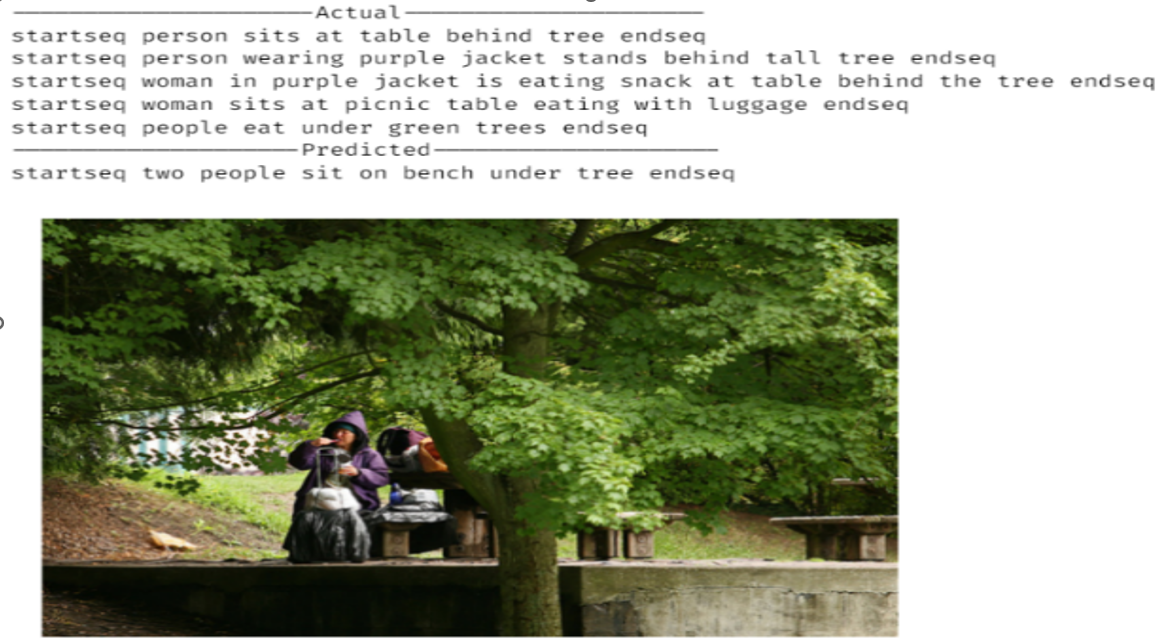
\includegraphics[width=0.9\linewidth]{result1}
\caption{Actual and predicted captions for image from the dataset}
\label{Fig:f2}
\end{center}
\end{figure}
\begin{figure}[H]
\begin{center}
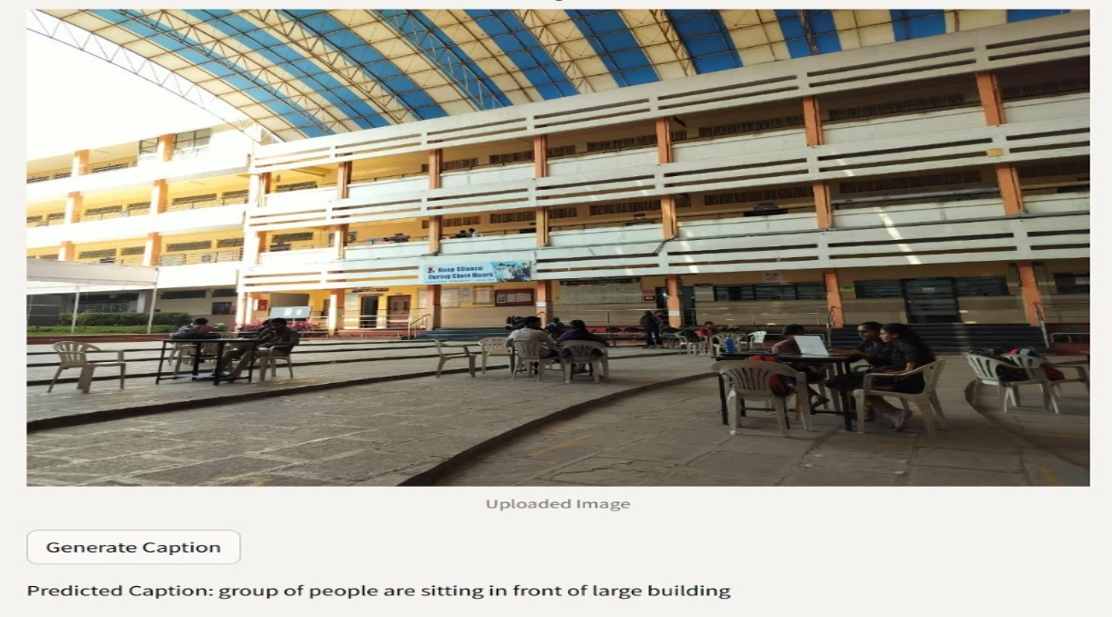
\includegraphics[width=0.8\linewidth]{result2}
\caption{Predicted caption for custom image}
\label{Fig:f2}
\end{center}
\end{figure}

\section{Performance evaluation}


\begin{table}[!htbp]
\begin{center}
\def\arraystretch{1.9}
  \begin{tabular}{| c | c | c |}
\hline
 \hspace{6.5mm}BLEU Metric \hspace{6.5mm} &	 \hspace{6.5mm}Flickr8k \hspace{6.5mm}&	 \hspace{6.5mm}Flickr30k \hspace{6.5mm} \\
\hline
BLEU-1 & 0.625841 & 0.598135\\
\hline





\end{tabular}
 \caption {Performance evaluation}
 \label{tab:CompAna}
\end{center}

\end{table}

\begin{figure}[H]
\begin{center}
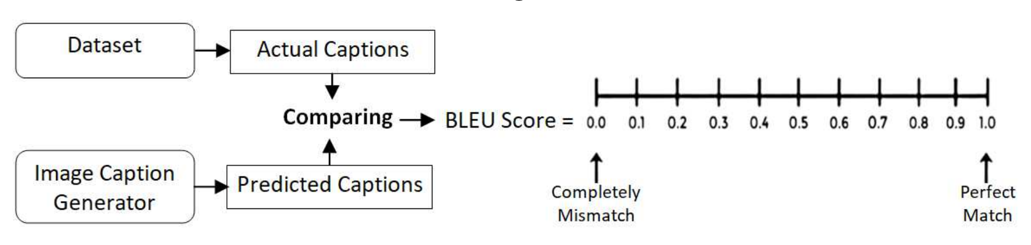
\includegraphics[width=0.8\linewidth]{performance}
\caption{The process of generating BLEU score}
\label{Fig:f2}
\end{center}
\end{figure}
The test set is used to predict picture captions, and these predictions are then evaluated using an established metric to evaluate the proposed model. BLEU ('Bilingual-Evaluation-Understudy'), a bilingual assessment metric, was used to gauge how effective the proposed photo captioning method was
to calculate BLEU score, a predicted sentence is compared to a reference sentence. The corresponding BLEU score prediction and examples of relevant captions are displayed. The Python NLTK module was used to produce the BLEU score for the evaluation of the candidate text. The quality of machine-generated versions is evaluated using the BLEU(Bilingual-Evaluation-Understudy) score. Phrase BLEU score for each sentence and Corpus BLEU Rating for groups of sentences are the two levels at which it works. Comparing comparable grammes in a preset order-for example, one gramme for single words and two grammes for word pairs-determines the N-gram scores. Every N-gram matche receives a weight, usually 0 for non-matches and one for matches. Balanced geometric averages of N-gram scores over a range of orders-from 1 to n-are computed to determine the BLUE score.The collective N-gram values (BLEU-N), which are produced by calculating the weighted geometrical average of the individaul N-gram scores, are a crucial facotr in determining the overall BLEU score.


\chapter{Advantages, Limitations and Application}
\section{Advantages}
\begin{itemize}
\item \textbf{Automated Description : }Deep learning models can automatically generate descriptive captions for images, reducing the need for manual annotation and providing textual information that can be used for various purposes.

\item \textbf{Accessibility :} Image captions can make visual content more accessible to individuals with visual impairments by providing descriptions of the content in a textual format.

\item \textbf{Content Retrieval :} Image captions can improve content retrieval in image databases or search engines. Users can search for images using text-based queries, making it easier to find specific images or content.

\item \textbf{Personalized Content : }Image captions can be tailored to the preferences or needs of the viewer. This personalization can enhance the user experience, especially in content recommendation systems.
\end{itemize}
\section{Limitations}
\begin{itemize}
\item \textbf{Accuracy and Quality : }Deep learning models for image captioning are not always perfect in generating accurate and high-quality captions. They can make mistakes, misinterpret images, or produce captions that do not accurately describe the content.

\item \textbf{Overfitting :} Deep learning models may overfit to the training data, which means they perform well on the training data but struggle with new or diverse images, leading to incorrect or irrelevant captions.
\item \textbf{Ambiguity Handling :} Images can be inherently ambiguous, and it can be challenging for deep learning models to handle ambiguity in image content and provide contextually appropriate captions.
\item \textbf{Lack of Common Sense Understanding :} Deep learning models often lack common sense reasoning abilities, which can lead to captions that make factual errors or provide implausible interpretations of images.
\end{itemize}
\section{Applications}
\begin{itemize}
\item \textbf{Social Media : }Image captioning is commonly used on social media platforms to automatically generate captions for user-uploaded images, making content more engaging and informative.
 \item \textbf{Content Recommendation : }Image captions can be used to personalize content recommendations by analyzing the textual descriptions and user preferences, improving user engagement and retention.
 \item \textbf{E-commerce : }Image captioning can provide product descriptions and details for e-commerce websites, enhancing the shopping experience by offering detailed information about products.
 \item \textbf{Education : }Image captioning can be applied in educational materials to provide additional context and information for images in textbooks, online courses, and educational websites.
\end{itemize}

\chapter{Summary and Conclusion}
\section{Summary}
Image captioning with EfficientNetV2 and a GRU is an advanced deep learning technique that enables automatic generation of descriptive text for images. EfficientNetV2, a convolutional neural network, extracts meaningful visual features from the input images. These features are then processed by a GRU, a type of recurrent neural network, to produce coherent and contextually relevant captions. This technology has a wide range of applications, including enhancing image accessibility for the visually impaired, automating image tagging, and improving content recommendation systems. It showcases the power of deep learning in bridging the gap between visual and textual information, ultimately facilitating more effective human-computer interactions and information retrieval.
\section{Conclusion}

In conclusion, image captioning using EfficientNetV2 and GRU represents a significant advancement in the field of deep learning. It demonstrates the ability of neural networks to comprehend and describe visual content with textual precision. The technology's applications in accessibility, image organization, and content recommendation underline its practical importance. As it continues to evolve, it has the potential to revolutionize how we interact with and understand the vast amount of visual data in today's digital world. Image captioning with EfficientNetV2 and GRU is a promising example of how artificial intelligence can enhance our relationship with visual media.
%\addcontentsline{toc}{chapter}{Bibliography}
%\newpage
%\vspace{10mm}
%{\fontsize{16}{15} \bfseries \LARGE \selectfont \centerline{Bibliography}}
\bibliographystyle{unsrt}
\bibliography{RishikeshTambe}

\begin{appendices}
% \chapter{ALGORITHMIC DESIGN}
\chapter{Awards/Participation in Project Competition/Exhibition}
Best Paper Award at ICRTACT 2024 for our research on image captioning using deep learning with GRU and EfficientNetV2 Novel Approach: Introduction of a novel methodology for image captioning that integrates GRU and EfficientNetV2, leveraging the strengths of both architectures to achieve superior performance.\\
\textbf{Experimental Results:} Presentation of comprehensive experimental results demonstrates the effectiveness and robustness of the proposed approach across various datasets and BLEU evaluation metrics. These results showcase the potential of our method to outperform existing techniques in the field.\\
\textbf{Technical Contributions:} Detailed description of the technical contributions, including model architecture, training strategies, hyperparameter tuning, and optimization techniques employed to enhance the performance of the image captioning system.\\
\textbf{Real-world Applications:} Discussed the potential real-world applications and implications of the proposed image captioning system, highlighting its relevance in areas such as assistive technology, content generation, and multimedia indexing.\\
\textbf{Future Directions:} Identified the future research directions and opportunities for further improving the proposed methodology, addressing challenges, and advancing the state-of-the-art in image captioning technology.

\chapter{Details of the Papers Publication (if any)}
\section{PAPER PUBLICATION IN UGC CARE GENERAL}

Publishing a paper in a UGC Care-listed journal indicates that our research has undergone a rigorous peer-review process and has been recognized for its quality and contribution to the field. 
\textbf{Title:} Image Captioning using EfficientNetV2 based on Encoder-Decoder Framework\\ 
\textbf{Authors:} Dr. Rahul Gaikwad, Mr. Mayur Gadakh, Mr. Gaurav Chaudhari, Ms. Akanksha Gaikwad, Ms. Shivanjali Dhage\\
\textbf{Journal Name:} UGC Care (paper number - 356)\\
\textbf{Publication Date:} 25/4/2024\\
\textbf{Abstract:} - In this work, a deep neural network-based framework consisting of a "Gated Recurrent Unit (GRU)" decoder and an “EfficientNetV2B0-based Convolutional Neural Network (CNN)” encoder is used to offer a unique method of automatic picture captioning. The framework is designed to perceive information points within images and their contextual relationships, facilitating the generation of meaningful and contextually relevant captions. The CNN encoder built on the EfficientNetV2B0 architecture is very good at identifying objects in pictures and extracting features while preserving spatial information. Next, a language describing the visual information collected in the photographs is created using these qualities. To improve the captioning process, the GRU decoder is essential in word prediction and sentence construction using the retrieved characteristics. The suggested neural network system combines the GRU model with the effectiveness and precision of the EfficientNetV2B0 model as an image feature extractor to provide fixed-length output vectors for ultimate predictions. Popular open-source datasets like Flickr-8k and Flickr-30k are used in the study to train and evaluate the model. Using Python-Keras and TensorFlow backend, the framework is implemented, demonstrating the effectiveness of the GRUbased model and EfficientNetV2B0 in automatic picture captioning tasks. The suggested method for producing correct and contextually appropriate picture captions is shown to be successful and accurate when performance evaluation is carried out using the BLEU (BiLingual Evaluation Understudy) measure.\\
\textbf{Keywords:} - Image Captioning, Convolutional Neural Networks (CNN), EfficientNetV2, Gated Recurrent Unit (GRU), Recurrent Neural Network (RNN).\\
\textbf{References:} Rahman, Md Mijanur, Ashik Uzzaman, and Sadia Islam Sami. "Implementing Deep Neural Network Based Encoder-Decoder Framework for Image Captioning." In 2021 IEEE International Conference on Signal Processing, Information, Communication \& Systems (SPICSCON), pp. 26-31. IEEE, 2021.\\


\chapter{Plagiarism Report For this Report}


\begin{figure}[H]
\begin{center}
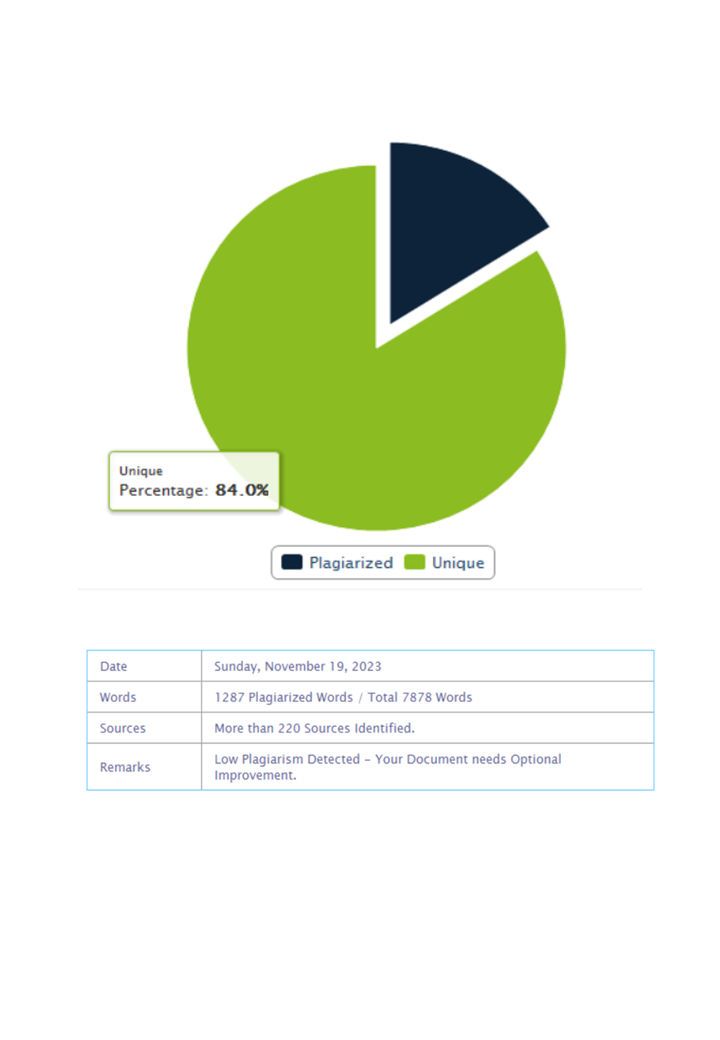
\includegraphics[width=1.0\linewidth]{plagfinal}
\end{center}
\end{figure}  

\chapter{Any other Documentation evidences related to Project}
\end{appendices}


\end{document}
